%!TEX root = ./main.tex
%
% This file is part of the i10 thesis template developed and used by the
% Media Computing Group at RWTH Aachen University.
% The current version of this template can be obtained at
% <http://www.media.informatik.rwth-aachen.de/karrer.html>.

\documentclass[11pt, a4paper, titlepage]{book}

% ! ACHTUNG !
% Nach dem ersten LaTeX durchlauf auf der Kommandozeile
% makeindex -s main.ist main.idx
% ausf�hren, sonst wird der Index nicht so sch�n formatiert.
% Leider macht TeXShop den makeindex Aufruf nur ohne Parameter.

% !ATTENTION!
% After running LaTeX for the first time using this template call
% makeindex -s main.ist main.idx
% to get the correct formatting for the index.

%Pakete und eigene Befehle - am besten durchlesen!
%Includes all neccessary packets and contains some useful commands - read this file!
%!TEX root = ./main.tex

% This file is part of the i10 thesis template developed and used by the
% Media Computing Group at RWTH Aachen University.
% The current version of this template can be obtained at
% <http://www.media.informatik.rwth-aachen.de/karrer.html>.



%-----------------------------------------------------------------------------------------------------------------------------------------
% Befehle
% commands
%-----------------------------------------------------------------------------------------------------------------------------------------

%----------------------------------------------------------------------------------
% \myBigFigure	[ LABEL_PREFIX (optional) ]
%				{ FILENAME (without extension) }
%				{ CAPTION TEXT }
%				{ SHORT VERSION OF CAPTION TEXT }
%
%Bild wird in kompletter Breite gesetzt, die Kurzversion der Bildunterschrift erscheint im Abbildungsverzeichnis
%picture using full width of the page, the short caption is what appears in the list of figures index

%----------------------------------------------------------------------------------
% \myFrameBigFigure	[ LABEL_PREFIX (optional) ]
%					{ FILENAME (without extension) }
%					{ CAPTION TEXT }
%					{ SHORT VERSION OF CAPTION TEXT }
%
%Bild wird in kompletter Breite gesetzt und eingerahmt, die Kurzversion der Bildunterschrift erscheint im Abbildungsverzeichnis
%picture with frame using the full width of the page, the short caption is what appears in the list of figures index

%----------------------------------------------------------------------------------
% \myHUGEFigure	[ LABEL_PREFIX (optional) ]
%				{ FILENAME (without extension) }
%				{ CAPTION TEXT }
%				{ SHORT VERSION OF CAPTION TEXT }
%
%Bild wird rotiert und quer in kompletter Breite gesetzt, die Kurzversion der Bildunterschrift erscheint im Abbildungsverzeichnis
%landscape picture using the full width of the rotated page, the short caption is what appears in the list of figures index

%----------------------------------------------------------------------------------
% \myFigure	[ LABEL_PREFIX (optional) ]
%			{ FILENAME (without extension) }
%			{ CAPTION TEXT }
%			{ SHORT VERSION OF CAPTION TEXT }
%
%Bild wird in der Breite der textspalte gesetzt, die Kurzversion der Bildunterschrift erscheint im Abbildungsverzeichnis
%picture using the width of the text column, the short caption is what appears in the list of figures index

%----------------------------------------------------------------------------------
% \myImgRef	[ LABEL_PREFIX (optional) ]
%			{ LABEL OF THE IMAGE }
%
%referenziert das angegebene Bild
%reference to an image

%----------------------------------------------------------------------------------
% \myBigTable	{ YOUR TABULAR DEFINITION }
%			{ CAPTION TEXT }
%			{ TABLE_LABLE }
%
%Tabelle wird in kompletter Breite gesetzt
%table using the full width of the page

%----------------------------------------------------------------------------------
% \myTable	{ YOUR TABULAR DEFINITION }
%			{ CAPTION TEXT }
%			{ TABLE_LABLE }
%
%Tabelle wird in der Breite der Textspalte gesetzt
%table using the width of the text column

%----------------------------------------------------------------------------------
% \myTxtRef	{ LABLE }
%
%Referenz auf Kapitel oder Abschnitte - gibt nummer und namen aus, z.B.: 5.3---"Yaddahyaddah"
%references chapters or sections, outputs number and title, e.g., 5.3---"Yaddahyaddah"

%----------------------------------------------------------------------------------
% \myUnderscore
%
%Setzt einen "sch�nen" Unterstrich f�r URLs
%typesets a 'nice' underscore for URLs

%----------------------------------------------------------------------------------
%\myTilde
%
%Setzt eine "sch�ne" Tilde f�r URLs
%typesets a 'nice' tilde for URLs

%----------------------------------------------------------------------------------
% \myURL	{ TYPESET VERSION OF ANCHOR }
%			{ PRISTINE URL }
%			{ TYPESET VERSION OF URL }
%
%Setzt eine URL
%die typographisch "sch�ne" version erscheint in einer Fu�note,
%im Text erscheint der Ankertext, verlinkt ist die "echte" URL
%typesets a URL
%the typographically correct version appears as a footnote,
%the anchor appears in the text, the link points to the pristine URL

%----------------------------------------------------------------------------------
% \mySimpleURL	{ TYPESET VERSION OF ANCHOR }
%				{ PRISTINE URL }
%
%Setzt eine URL
%die URL erscheint in einer Fu�note,
%im Text erscheint der Ankertext, die URL ist verlinkt
%typesets a URL
%the URL appears as a footnote,
%the anchor appears in the text, the link points to the URL

%----------------------------------------------------------------------------------
% \myProjectURL	{ TYPESET VERSION OF ANCHOR }
%				{ PRISTINE URL INSIDE PROJECT DIRECTORY }
%				{ TYPESET VERSION OF URL INSIDE PROJECT DIRECTORY }
%
%Setzt eine URL innerhalb des Projektverzeichnisses auf "media"
%ACCOUNT muss durch den eigenen Usernamen ersetzt werden
%die typographisch "sch�ne" version erscheint in einer Fu�note,
%im Text erscheint der Ankertext, verlinkt ist die "echte" URL
%typesets a URL inside the project directory on 'media'
%replace ACCOUNT with your username
%the typographically correct version appears as a footnote,
%the anchor appears in the text, the link points to the pristine URL

%----------------------------------------------------------------------------------
% \mnote	{ MARGIN NOTE }
%
%Setzt eine Randnotitz
%puts a comment into the margin in small sans-serif font

%----------------------------------------------------------------------------------
% \todo	{ TODO MARGIN NOTE }
%
%Setzt eine "ToDo"-Randnotitz in rot zur Erinnerung
%puts a 'todo' comment into the margin in red

%----------------------------------------------------------------------------------
% \chapterquote	{ QUOTATION }
%				{ SOURCE }
%
%Setzt ein Zitat zum Einleiten eines Kapitels
%outputs a quote with its source, can be used as an introduction to chapters

%----------------------------------------------------------------------------------
% \myDefBox	{ TERM }
%			{ DEFINITION }
%
%Setzt eine Randnotitz und eine farbige Box (Textspaltenbreite),
%welche einen Begriff und seine Definition enth�lt
%outputs a margin note and a colored box (width of the text column) containing a term and its definition

%----------------------------------------------------------------------------------
% \myBigDefBox	{ TERM }
%				{ DEFINITION }
%
%Setzt eine farbige Box (Seitenbreite), welche einen Begriff und seine Definition enth�lt
%outputs a colored box (width of the page) containing a term and its definition

%----------------------------------------------------------------------------------
% \myDownloadURL	{ TYPESET DOWNLOAD NAME }
%					{ PRISTINE VERSION OF FILENAME }
%					{ TYPESET VERSION OF FILENAME }
%
%Setzt eine farbige Box, welche einen Downloadlink enth�lt
%outputs a colored box containing a download link

%----------------------------------------------------------------------------------
% \emptydoublepage
%
% Leere Doppelseite ohne Kopf- oder Fu�zeile am Ende von Kapiteln
% Clear double page without any header or footer at end of chapters

%----------------------------------------------------------------------------------
% \pagebreak	[ SOME STRANGE LATEX VALUE ]
%
%Eklige pagebreaks f�r den Druck (falls es nicht mehr anders geht)
%pagebreaks for the final print version (last resort weapon against wrong pagebreaks by LaTeX)

%----------------------------------------------------------------------------------
% \TM
%
%Setzt ein (TM) Symbol
%Places a (TM) symbol


%----------------------------------------------------------------------------------
%Packages and parameters
%----------------------------------------------------------------------------------

%Inputencoding f�r den Mac
%inputencoding for the mac
\usepackage[utf8]{inputenc}

%Mathe- und Symbolpakete
%packages for mathematical symbols
\usepackage{latexsym}
\usepackage{amsmath}
\usepackage{amssymb}

%Tabellengestaltung
%table design
\usepackage{booktabs}

%Grafikpaket
%grahics package
\usepackage{color,graphicx}

%relativer Pfad zu den Bildern
%path to your image folder
\graphicspath{{images/}}

%Abs�tze werden nicht eingezogen, sondern vertikal abgesetzt
%do not indent at new paragraphs but add a vertical offset
\usepackage{noindent}

%Palatino+Helvetica statt Computer Modern als standard fonts:
%change standard fonts to Palatino and Helvetica
\usepackage{palatino}

%Bibliographieeinstellungen
%bibliography settings
\usepackage{natbib}
\bibliographystyle{plainnat}

%Zitierbefehle
%citation commands
\newcommand{\fullcite}{\citep} %for "Author [1980]"
\renewcommand{\citeyear}{\citeyearpar} %for "[1980]"

%paket f�r erweiterte kontrollstrukturen
%package for control structures
\usepackage{ifthen}

%marginpar hack --- alle Randnotitzen sollten dann auf der richtigen Seite stehen
%marginpar hack --- moves margin notes to correct position
\usepackage{mparhack}

%lesbare verweise
%make readable references
\usepackage[pdftex,plainpages=false,pdfpagelabels]{hyperref}


%---------------------<Layout in the style of "A Pattern Approach to Interaction Design>---------------------------

% Change page headers and footers:
\usepackage{fancyhdr}
\pagestyle{fancy}
\fancyhf{}
\fancyhead[RE]{\slshape \nouppercase{\leftmark}}    % Even page header: "page   chapter"
\fancyhead[LO]{\slshape \nouppercase{\rightmark}}   % Odd  page header: "section   page"
\fancyhead[RO,LE]{\bfseries \thepage} 
\renewcommand{\headrulewidth}{1pt}    % Underline headers
\renewcommand{\footrulewidth}{0pt}    

\fancypagestyle{plain}{               % No chapter+section on chapter start pages
\fancyhf{}
\fancyhead[RO,LE]{\bfseries \thepage}
\renewcommand{\headrulewidth}{1pt}
\renewcommand{\footrulewidth}{0pt}
}

% Left headings: "1  INTRODUCTION"
\renewcommand{\chaptermark}[1]{%
\markboth{\thechapter\ \ \ \ #1}{}}

% Right headings: "1.1  Basics"
\renewcommand{\sectionmark}[1]{%
\markright{\thesection\ \ \ \ #1}{}}

% some Fancyhdr problem...
\addtolength{\headheight}{2pt} % To avoid overfull vboxes from fancyhdr


%creating a better way to change the layout for the abstract pages
\usepackage{geometry}

\ifthenelse{\lengthtest{\paperheight=250mm}}%
{% -----------------B5 Layout-----------------
% Page layout

%\pdfpageheight250mm
%\pdfpagewidth176mm
\geometry{	b5paper,
			top = 27mm,
			footskip = 10mm,
			inner = 19mm,
			outer = 39mm,
			textheight = 175mm,
			textwidth = 84mm,
			marginparsep = 3mm,
			marginparwidth = 32mm
}
\savegeometry{myText}
% -----------------/ B5 Layout-----------------
}%
{% -----------------A4 Layout-----------------
% Page layout
\geometry{	a4paper,
			twoside,
			includemp,
			includehead,
			top = 30mm,
			headsep = 10mm,
			bindingoffset = 10mm,
			inner = 20mm,
			outer = 40mm,
			bottom = 45mm,
			marginparsep = 10mm,
			marginparwidth = 30mm
}
\savegeometry{myText}
% -----------------/ A4 Layout-----------------
}
% Abstract layout
\geometry{	marginparsep = 0mm,
			marginparwidth = 0mm
}
\savegeometry{myAbstract}
\loadgeometry{myText}

\newlength{\fullwidth} % Width of text plus margin notes
\setlength{\fullwidth}{\textwidth}
\addtolength{\fullwidth}{\marginparsep}
\addtolength{\fullwidth}{\marginparwidth}

\setlength{\headwidth}{\fullwidth} % Header stretches over margin notes


%---------------------</Layout in the style of "A Pattern Approach to Interaction Design>---------------------------


%wird f�r die fl�chendeckende Ausgabe der Titelseite ben�tigt
%needed for the full-face titlepage
\usepackage{eso-pic}

%index verwenden
%make an index
\usepackage{makeidx}
\makeindex

%Index Formatierungshilfen
%formatting helpers for the index
\newcommand{\uu}[1]{\underline{#1}}
\newcommand{\ii}[1]{\textit{#1}}

%neue Definition der Index Umgebung
%redesign of the index
\renewenvironment{theindex}{%
  \vspace*{50pt}%
  {\Huge\bfseries\indexname}\par%
  \vspace*{40pt}%
  \setlength{\parskip}{0pt}%
  \setlength{\parindent}{0pt}%
  \small%
  \renewcommand{\item}{\par{}}%
  \renewcommand{\subitem}{\par\hspace{2em}- }%
}%
{}

%Maximale Gliederungstiefe, die noch ins Inhaltsverzeichnis aufgenommen wird
%maximum depth for the table of contents
\setcounter{tocdepth}{3}

%Vorschlag f�r ein sch�nes Farbschema
%Set of colors which look nice together
\usepackage{color}
\definecolor{orange_light}{rgb}{1,0.8,0.4}
\definecolor{orange_med}{rgb}{0.753,0.62,0.373}
\definecolor{orange_dark}{rgb}{0.506,0.412,0.251}

\definecolor{green_light}{rgb}{0.8,1,0.4}
\definecolor{green_med}{rgb}{0.635,0.745,0.376}
\definecolor{green_dark}{rgb}{0.435,0.498,0.255}

\definecolor{blue_light}{rgb}{0.4,0.8,1}
\definecolor{blue_med}{rgb}{0.365,0.624,0.749}
\definecolor{blue_dark}{rgb}{0.251,0.42,0.502}

\definecolor{pink_light}{rgb}{1,0.435,0.812}
\definecolor{pink_med}{rgb}{0.745,0.38,0.62}
\definecolor{pink_dark}{rgb}{0.498,0.255,0.416}

\definecolor{yellow_light}{rgb}{1,1,0.4}
\definecolor{yellow_med}{rgb}{0.757,0.745,0.373}
\definecolor{yellow_dark}{rgb}{0.506,0.49,0.251}

%blau (f�r URLs)
%blue (for URLs)
\definecolor{blue}{rgb}{0,0,1}

%notwendig f�r die korrekte Erkennung, auf welcher Seite sich eine Abbildung befindet.
%we need this to determine if a figure is on an odd or even page
\usepackage{chngpage}

%Hiermit k�nnen die Abbildungslegenden frei gestaltet werden
%we need this to redesign the captions
\usepackage[font=normalsize,labelfont=bf]{caption}

%Abbildungen kommen auf eine eigene Seite, wenn sie mehr als 85% des Platzes
%auf einer Seite einnehmen
%if a figure takes more than 85% of a page it will be typeset on a separate page
\renewcommand{\floatpagefraction}{0.85}

%Ben�tigt um gro�e Abbildungen gedreht auf eine Seite zu setzen
%we need this to rotate big figures
\usepackage[figuresright]{rotating}

%Verschiedene L�ngenma�e f�r Textboxen
%dimensions for textboxes
\newlength{\myDefBoxWidth}
\setlength{\myDefBoxWidth}{\textwidth}
\addtolength{\myDefBoxWidth}{-4mm}
\newlength{\myBigDefBoxWidth}
\setlength{\myBigDefBoxWidth}{\fullwidth}
\addtolength{\myBigDefBoxWidth}{-4mm}

%Formathilfen f�r MatLab Code (wer's braucht...)
%pre-defined matlab code formats
\usepackage{alltt}
\definecolor{string}{rgb}{0.7,0.0,0.0}
\definecolor{comment}{rgb}{0.13,0.54,0.13}
\definecolor{keyword}{rgb}{0.0,0.0,1.0}



%-----------------------------------------------------------------------------------------------------------------------------------------
% neue Befehle
% new commands
%-----------------------------------------------------------------------------------------------------------------------------------------

%----------------------------------------------------------------------------------
% \myBigFigure	[ LABEL_PREFIX (optional) ]
%				{ FILENAME (without extension) }
%				{ CAPTION TEXT }
%				{ SHORT VERSION OF CAPTION TEXT }
%
%Bild wird in kompletter Breite gesetzt
%picture using full width of the page
\newcommand{\myBigFigure}[4][image]
{%
\begin{figure}[t!bp]%
	\checkoddpage%
	\ifcpoddpage%
		%nothing
	\else
		\hspace{-\marginparsep}\hspace{-\marginparwidth}%
	\fi
	%use minipage to center the label beneath the figure
	\begin{minipage}{\fullwidth}%
		\includegraphics[width= \fullwidth]{#2}%
		\caption[#4]{#3}%
		\label{#1_#2}%
	\end{minipage}%
\end{figure}%
}


%----------------------------------------------------------------------------------
% \myFrameBigFigure	[ LABEL_PREFIX (optional) ]
%					{ FILENAME (without extension) }
%					{ CAPTION TEXT }
%					{ SHORT VERSION OF CAPTION TEXT }
%
%Bild wird in kompletter Breite gesetzt und eingerahmt
%picture with frame using the full width of the page
\newcommand{\myFrameBigFigure}[4][image]
{
\begin{figure}[t!bp]
	\checkoddpage
	\ifcpoddpage
		%nothing
	\else
		\hspace{-\marginparsep}\hspace{-\marginparwidth}
	\fi
	%use minipage to center the label beneath the figure
	\begin{minipage}{\fullwidth}
	\frame{%
		\includegraphics[width= \fullwidth]{#2}%
		}
		\caption[#4]{#3}
		\label{#1_#2}
	\end{minipage}
\end{figure}
}

%----------------------------------------------------------------------------------
% \myHUGEFigure	[ LABEL_PREFIX (optional) ]
%				{ FILENAME (without extension) }
%				{ CAPTION TEXT }
%				{ SHORT VERSION OF CAPTION TEXT }
%
%Bild wird rotiert und quer in kompletter Breite gesetzt
%landscape picture using the full width of the rotated page
\newcommand{\myHugeFigure}[4][image]
{
\begin{sidewaysfigure}[t!bp]
	\checkoddpage
	\ifcpoddpage
		%nothing
		\vspace{\marginparsep}\vspace{\marginparwidth}
	\else
		%nothing
		\vspace{-\marginparsep}\vspace{-\marginparwidth}
	\fi
		\includegraphics[width= \textheight]{#2}
		\caption[#4]{#3}
		\label{#1_#2}
	
\end{sidewaysfigure}
}

%----------------------------------------------------------------------------------
% \myFigure	[ LABEL_PREFIX (optional) ]
%			{ FILENAME (without extension) }
%			{ CAPTION TEXT }
%			{ SHORT VERSION OF CAPTION TEXT }
%
%Bild wird in der Breite der textspalte gesetzt
%picture using the width of the text column
\newcommand{\myFigure}[4][image]%
{%
\begin{figure}[t!bp]%
	\begin{center}%
		\includegraphics[width= \textwidth]{#2}%
		\caption[#4]{#3}
		\label{#1_#2}%
	\end{center}%
\end{figure}%
}%

%----------------------------------------------------------------------------------
% \myImgRef	[ LABEL_PREFIX (optional) ]
%			{ LABEL OF THE IMAGE }
%
%referenziert das angegebene Bild
%reference to an image
\newcommand{\myImgRef}[2][image]%
{%
	\ref{#1_#2}%
}%

%----------------------------------------------------------------------------------
% \myBigTable	{ YOUR TABULAR DEFINITION }
%			{ CAPTION TEXT }
%			{ TABLE_LABLE }
%
%Tabelle wird in kompletter Breite gesetzt
%table using the full width of the page
\newcommand{\myBigTable}[3]%
{%
\begin{table}[htdp]%
	\checkoddpage%
	\ifcpoddpage%
		%nothing
	\else%
		\hspace{-\marginparsep}\hspace{-\marginparwidth}%
	\fi%
	\begin{minipage}{\fullwidth}%
		\begin{center}%
			#1%
			\caption{#2}%
			\label{#3}%
		\end{center}%	
	\end{minipage}%
\end{table}%
}%

%----------------------------------------------------------------------------------
% \myTable	{ YOUR TABULAR DEFINITION }
%			{ CAPTION TEXT }
%			{ TABLE_LABLE }
%
%Tabelle wird in der Breite der Textspalte gesetzt
%table using the width of the text column
\newcommand{\myTable}[3]%
{%
\begin{table}[htdp]%
	\begin{center}%
		#1%
		\caption{#2}%
		\label{#3}%
	\end{center}%	
\end{table}%
}%

%----------------------------------------------------------------------------------
% \myTxtRef	{ LABLE }
%
%Referenz auf Kapitel oder Abschnitte - gibt nummer und namen aus, z.B.: 5.3---"Yaddahyaddah"
%references chapters or sections, outputs number and title, e.g., 5.3---"Yaddahyaddah"
\newcommand{\myTxtRef}[1]
{%
	\ref{#1} ``\nameref{#1}''%
}

%----------------------------------------------------------------------------------
% \myTxtRefPP	{ LABLE }
%
%Referenz auf Kapitel oder Abschnitte - gibt nummer, namen und seiten aus, z.B.: 5.3---"Yaddahyaddah" (p. 45)
%references chapters or sections, outputs number and title, e.g., 5.3---"Yaddahyaddah"
\newcommand{\myTxtRefPP}[1]
{%
	\ref{#1} ``\nameref{#1}'' (p.~\pageref{#1})%
}

%----------------------------------------------------------------------------------
% \myUnderscore
%
%Setzt einen "sch�nen" Unterstrich f�r URLs
%typesets a 'nice' underscore for URLs
\newcommand{\myUnderscore}{$\underline{\hspace{0.5em}}$}

%----------------------------------------------------------------------------------
%\myTilde
%
%Setzt eine "sch�ne" Tilde f�r URLs
%typesets a 'nice' tilde for URLs
\newcommand{\myTilde}{$\sim$}

%----------------------------------------------------------------------------------
% \myURL	{ TYPESET VERSION OF ANCHOR }
%			{ PRISTINE URL }
%			{ TYPESET VERSION OF URL }
%
%Setzt eine URL
%die typographisch "sch�ne" version erscheint in einer Fu�note,
%im Text erscheint der Ankertext, verlinkt ist die "echte" URL
%typesets a URL
%the typographically correct version appears as a footnote,
%the anchor appears in the text, the link points to the pristine URL
\newcommand{\myURL}[3]%
{%
	\textcolor{blue}{%
		\href{#2}{#1}%
	}%
	\footnote{#3}%
}

%----------------------------------------------------------------------------------
% \mySimpleURL	{ TYPESET VERSION OF ANCHOR }
%				{ PRISTINE URL }
%
%Setzt eine URL
%die URL erscheint in einer Fu�note,
%im Text erscheint der Ankertext, die URL ist verlinkt
%typesets a URL
%the URL appears as a footnote,
%the anchor appears in the text, the link points to the URL
\newcommand{\mySimpleURL}[2]%
{%
	\textcolor{blue}{%
		\href{#2}{#1}%
	}%
	\footnote{#2}%
}

%----------------------------------------------------------------------------------
% \myProjectURL	{ TYPESET VERSION OF ANCHOR }
%				{ PRISTINE URL INSIDE PROJECT DIRECTORY }
%				{ TYPESET VERSION OF URL INSIDE PROJECT DIRECTORY }
%
%Setzt eine URL auf hci/public wo die Inhalte des WebServer Ordners auf "oliver" verf�gbar sind
%die typographisch "sch�ne" version erscheint in einer Fu�note,
%im Text erscheint der Ankertext, verlinkt ist die "echte" URL
%typesets a URL to hci/public from where the contents of the WebServer folder from oliver can be accessed
%the typographically correct version appears as a footnote,
%the anchor appears in the text, the link points to the pristine URL
\newcommand{\myProjectURL}[3]%
{%
	\textcolor{blue}{%
		\href{http://hci.rwth-aachen.de/public/#2}{#1}%
	}%
	\footnote{http://hci.rwth-aachen.de/public/#3}%
}

%----------------------------------------------------------------------------------
% \mnote	{ MARGIN NOTE }
%
%Setzt eine Randnotitz
%puts a comment into the margin in small sans-serif font
\newcommand{\mnote}[1]%
{%
	\leavevmode%
	\checkoddpage%
	\ifcpoddpage%
		\marginpar{\raggedright\textsf{{\footnotesize{#1}}}}%
	\else%
		\marginpar{\raggedleft\textsf{{\footnotesize{#1}}}}%
	\fi%
}
	
% leavevmode allows mnotes to be aligned with the first line of a paragraph
% NOTE: you have to put a "%" at the end of the line with the mnote, or you will get an extra blank at the beginning of the paragraph!

%----------------------------------------------------------------------------------
% \todo	{ TODO MARGIN NOTE }
%
%Setzt eine "ToDo"-Randnotitz in rot zur Erinnerung
%puts a 'todo' comment into the margin in red
\definecolor{red}{rgb}{1,0,0}
\newcommand{\todo}[1]{\mnote{\textcolor{red}{ToDo: #1}}}

%----------------------------------------------------------------------------------
% \chapterquote	{ QUOTATION }
%				{ SOURCE }
%
%Setzt ein Zitat zum Einleiten eines Kapitels
%outputs a quote with its source, can be used as an introduction to chapters
\newcommand{\chapterquote}[2]{
\begin{quotation}
    \begin{flushright}
	\noindent\emph{``{#1}''\\[1.5ex]---{#2}}
    \end{flushright}
\end{quotation}
}

%----------------------------------------------------------------------------------
% \myDefBox	{ TERM }
%			{ DEFINITION }
%
%Setzt eine Randnotitz und eine farbige Box (Textspaltenbreite),
%welche einen Begriff und seine Definition enth�lt
%outputs a margin note and a colored box (width of the text column) containing a term and its definition
\newcommand{\myDefBox}[2]
{%
	\setlength{\fboxrule}{1mm}%
	\fcolorbox{orange_med}{orange_light}%
	{%
		\parbox{\myDefBoxWidth}{{\bfseries\scshape#1:}\\#2}%
	}%
	\mnote{Definition:\\\emph{#1}}
}

%----------------------------------------------------------------------------------
% \myBigDefBox	{ TERM }
%				{ DEFINITION }
%
%Setzt eine farbige Box (Seitenbreite), welche einen Begriff und seine Definition enth�lt
%outputs a colored box (width of the page) containing a term and its definition
\newcommand{\myBigDefBox}[2]
{%
	\begin{figure}[h!]
	\setlength{\fboxrule}{1mm}%
	\checkoddpage%
	\ifcpoddpage%
		%nothing
	\else%
		\hspace{-\marginparsep}\hspace{-\marginparwidth}%
	\fi%
	\fcolorbox{orange_med}{orange_light}%
	{%
		\parbox{\myBigDefBoxWidth}{{\bfseries\scshape#1:}\\#2}%
	}%
	\end{figure}
}

%----------------------------------------------------------------------------------
% \myDownloadURL	{ TYPESET DOWNLOAD NAME }
%					{ PRISTINE VERSION OF FILENAME }
%					{ TYPESET VERSION OF FILENAME }
%
%Setzt eine farbige Box, welche einen Downloadlink enth�lt
%outputs a colored box containing a download link
\newcommand{\myDownloadURL}[3]{%
\checkoddpage%
	\ifcpoddpage%
		%nothing
	\else%
		\hspace{-\marginparsep}\hspace{-\marginparwidth}%
	\fi%
\setlength{\fboxrule}{1mm}%
\fcolorbox{green_med}{green_light}{%
\begin{minipage}{\myBigDefBoxWidth}%
\begin{center}%
\myProjectURL{#1}{folder/#2}{folder/#3}%
\end{center}%
\end{minipage}%
}%
}

%----------------------------------------------------------------------------------
% \emptydoublepage
%
% Leere Doppelseite ohne Kopf- oder Fu�zeile am Ende von Kapiteln
% Clear double page without any header or footer at end of chapters
\newcommand{\emptydoublepage}{\clearpage\thispagestyle{empty}\cleardoublepage}

%----------------------------------------------------------------------------------
% \pagebreak	[ SOME STRANGE LATEX VALUE ]
%
%Eklige pagebreaks f�r den Druck (falls es nicht mehr anders geht)
%pagebreaks for the final print version (last resort weapon against wrong pagebreaks by LaTeX)
\newcommand{\PB}[1][3]
{%
	\pagebreak[#1]%
}



%----------------------------------------------------------------------------------
% \TM
%
%Setzt ein (TM) Symbol
%Places a (TM) symbol
\newcommand{\TM}
{%
	\textsuperscript{\texttrademark}%
}

\usepackage{listings}
\usepackage{color}
\usepackage{array}
\usepackage{varwidth}


%--------------------------------------------------------------
%Dokumentspezifisches
%Stuff regarding your specific document
%--------------------------------------------------------------

%Trennungshilfen
%Hyphenation patterns
\hyphenation{
dieseswortwirdnichtgetrennt
diesesauchnicht
thiswordwillstayinoneline
thistoo
}


%--------------------------------------------------------------
\begin{document}

% gr��ere Wortabst�nde zulassen, um Trennungen zu vermeiden
% allow more flexible whitespaces to avoid hyphenation and overfull hboxes
\sloppy

% "see" Eintr�ge f�r den Index
% 'see'-entries for the index
%!TEX root = ./main.tex
%
% This file is part of the i10 thesis template developed and used by the
% Media Computing Group at RWTH Aachen University.
% The current version of this template can be obtained at
% <http://www.media.informatik.rwth-aachen.de/karrer.html>.




%--------------------------------------------------------------
\frontmatter

%Die Titelseite aus dem "images"-Verzeichnis wird verwendet
%use the titlepage from the 'images' directory
%Bachelor's: titlepage_Bachelor
%Master's:   titlepage_Master
%Neutral:    titlepage
\begin{titlepage}
\AddToShipoutPicture*{
\put(0,0){

\includegraphics[width=\paperwidth]{titlepage_bachelor}}}
\strut
\end{titlepage}

\thispagestyle{empty}
\emptydoublepage

% This file is part of the i10 thesis template developed and used by the
% Media Computing Group at RWTH Aachen University.
% The current version of this template can be obtained at
% <http://www.media.informatik.rwth-aachen.de/karrer.html>.

% As of WS2015/16 the ZPA only accepts its own statement of oath: 

\begin{titlepage}
\AddToShipoutPicture*{
\put(0,0){
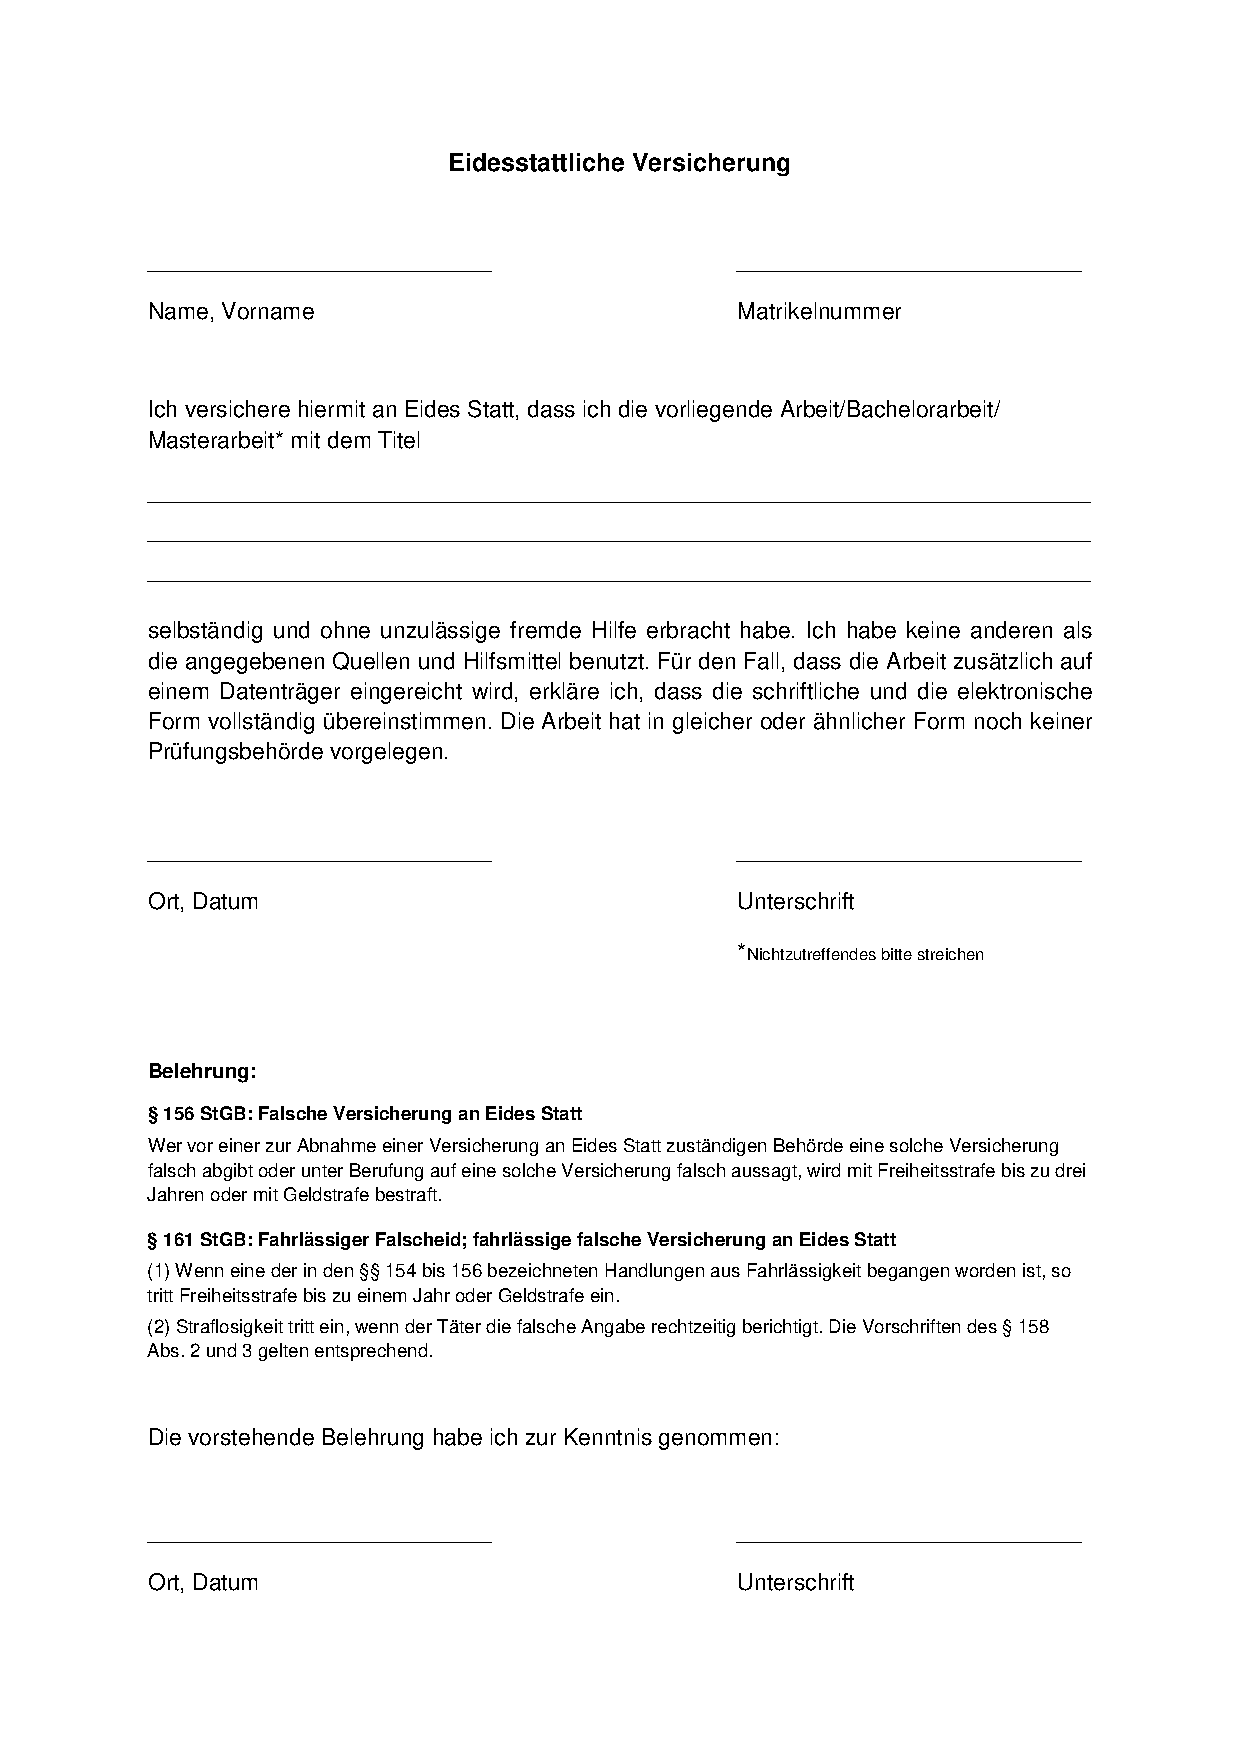
\includegraphics[width=\paperwidth]{oathstatement}}}
\strut
\end{titlepage}

% The following lines are depricated. Only uncomment them when your thesis is _not_ submitted to RWTH Aachen University. In this case, comment the lines 8–13 (above) in addition to remove the ZPA statement of oath.

%~
%\vfill
%I hereby declare that I have created this work completely on my own and used no other sources or tools than the ones listed, and that I have marked any citations accordingly.
%
%Hiermit versichere ich, dass ich die vorliegende Arbeit selbst\"andig verfasst und keine anderen als die angegebenen Quellen und Hilfsmittel benutzt sowie Zitate kenntlich gemacht habe. 
%
%\begin{flushright}
%\vspace{12mm}
%$\overline{Aachen, MONTH \mathit{YEAR}}$\\
%\textit{YOUR NAME}
%\end{flushright}

\emptydoublepage

\setcounter{page}{5}

\tableofcontents
\emptydoublepage
%
\listoffigures
\emptydoublepage
%
\listoftables
\emptydoublepage

%Die �bersicht sollte in englischer und in deutscher Sprache verfasst werden
%the abstract should include an english and a german version
%!TEX root = ./main.tex

% This file is part of the i10 thesis template developed and used by the
% Media Computing Group at RWTH Aachen University.
% The current version of this template can be obtained at
% <http://www.media.informatik.rwth-aachen.de/karrer.html>.

\loadgeometry{myAbstract}

\chapter*{Abstract\markboth{Abstract}{Abstract}}
\addcontentsline{toc}{chapter}{\protect\numberline{}Abstract}
\label{abstract}

%here (english version)
Lorem ipsum dolor sit amet, consectetur adipisicing elit, sed do eiusmod tempor incididunt ut labore et dolore magna aliqua. Ut enim ad minim veniam, quis nostrud exercitation ullamco laboris nisi ut aliquip ex ea commodo consequat. Duis aute irure dolor in reprehenderit in voluptate velit esse cillum dolore eu fugiat nulla pariatur. Excepteur sint occaecat cupidatat non proident, sunt in culpa qui officia deserunt mollit anim id est laborum.Lorem ipsum dolor sit amet, consectetur adipisicing elit, sed do eiusmod tempor incididunt ut labore et dolore magna aliqua. Ut enim ad minim veniam, quis nostrud exercitation ullamco laboris nisi ut aliquip ex ea commodo consequat. Duis aute irure dolor in reprehenderit in voluptate velit esse cillum dolore eu fugiat nulla pariatur. Excepteur sint occaecat cupidatat non proident, sunt in culpa qui officia deserunt mollit anim id est laborum.Lorem ipsum dolor sit amet, consectetur adipisicing elit, sed do eiusmod tempor incididunt ut labore et dolore magna aliqua. Ut enim ad minim veniam, quis nostrud exercitation ullamco laboris nisi ut aliquip ex ea commodo consequat. Duis aute irure dolor in reprehenderit in voluptate velit esse cillum dolore eu fugiat nulla pariatur. Excepteur sint occaecat cupidatat non proident, sunt in culpa qui officia deserunt mollit anim id est laborum.Lorem ipsum dolor sit amet, consectetur adipisicing elit, sed do eiusmod tempor incididunt ut labore et dolore magna aliqua. Ut enim ad minim veniam, quis nostrud exercitation ullamco laboris nisi ut aliquip ex ea commodo consequat. Duis aute irure dolor in reprehenderit in voluptate velit esse cillum dolore eu fugiat nulla pariatur. Excepteur sint occaecat cupidatat non proident, sunt in culpa qui officia deserunt mollit anim id est laborum.

\chapter*{\"Uberblick\markboth{\"Uberblick}{\"Uberblick}}
\addcontentsline{toc}{chapter}{\protect\numberline{}\"Uberblick}
\label{ueberblick}

%here (deutsche version)
Lorem ipsum dolor sit amet, consectetur adipisicing elit, sed do eiusmod tempor incididunt ut labore et dolore magna aliqua. Ut enim ad minim veniam, quis nostrud exercitation ullamco laboris nisi ut aliquip ex ea commodo consequat. Duis aute irure dolor in reprehenderit in voluptate velit esse cillum dolore eu fugiat nulla pariatur. Excepteur sint occaecat cupidatat non proident, sunt in culpa qui officia deserunt mollit anim id est laborum.Lorem ipsum dolor sit amet, consectetur adipisicing elit, sed do eiusmod tempor incididunt ut labore et dolore magna aliqua. Ut enim ad minim veniam, quis nostrud exercitation ullamco laboris nisi ut aliquip ex ea commodo consequat. Duis aute irure dolor in reprehenderit in voluptate velit esse cillum dolore eu fugiat nulla pariatur. Excepteur sint occaecat cupidatat non proident, sunt in culpa qui officia deserunt mollit anim id est laborum.Lorem ipsum dolor sit amet, consectetur adipisicing elit, sed do eiusmod tempor incididunt ut labore et dolore magna aliqua. Ut enim ad minim veniam, quis nostrud exercitation ullamco laboris nisi ut aliquip ex ea commodo consequat. Duis aute irure dolor in reprehenderit in voluptate velit esse cillum dolore eu fugiat nulla pariatur. Excepteur sint occaecat cupidatat non proident, sunt in culpa qui officia deserunt mollit anim id est laborum.Lorem ipsum dolor sit amet, consectetur adipisicing elit, sed do eiusmod tempor incididunt ut labore et dolore magna aliqua. Ut enim ad minim veniam, quis nostrud exercitation ullamco laboris nisi ut aliquip ex ea commodo consequat. Duis aute irure dolor in reprehenderit in voluptate velit esse cillum dolore eu fugiat nulla pariatur. Excepteur sint occaecat cupidatat non proident, sunt in culpa qui officia deserunt mollit anim id est laborum.


\loadgeometry{myText}

\emptydoublepage

%Danksagungen
%acknowledgements
%!TEX root = ./main.tex
%
% This file is part of the i10 thesis template developed and used by the
% Media Computing Group at RWTH Aachen University.
% The current version of this template can be obtained at
% <http://www.media.informatik.rwth-aachen.de/karrer.html>.

\loadgeometry{myAbstract}

\chapter*{Acknowledgements\markboth{Acknowledgements}{Acknowledgements}}
\addcontentsline{toc}{chapter}{\protect\numberline{}Acknowledgements}

%Put your acknowledgements in here.
Thank you!

\loadgeometry{myText}


\emptydoublepage

%In der Arbeit verwendete Konventionen (Formelsatz, Definitionen, etc.)
%conventions applied in the thesis (AE/BE, definitions, etc.)
%!TEX root = ./main.tex
%
% This file is part of the i10 thesis template developed and used by the
% Media Computing Group at RWTH Aachen University.
% The current version of this template can be obtained at
% <http://www.media.informatik.rwth-aachen.de/karrer.html>.

\chapter*{Conventions\markboth{Conventions}{Conventions}}
\addcontentsline{toc}{chapter}{\protect\numberline{}Conventions}

Throughout this thesis we use the following conventions.



\bigskip

\emph{Text conventions}

Definitions of technical terms or short excursus are set off in coloured boxes.

\myDefBox{Excursus}
{Excursus are detailed discussions of a particular point in a book, usually in an appendix, or digressions in a written text.}

\medskip

Source code and implementation symbols are written in typewriter-style text.

\texttt{myClass}

\medskip

The whole thesis is written in Canadian English.

\medskip

Download links are set off in coloured boxes.

\myDownloadURL{File: myFile}{file_number.file}{file\myUnderscore number.file}

%\pagebreak

%\emph{Formula conventions}




\emptydoublepage

%--------------------------------------------------------------
\mainmatter

%!TEX root = ./main.tex
%
% This file is part of the i10 thesis template developed and used by the
% Media Computing Group at RWTH Aachen University.
% The current version of this template can be obtained at
% <http://www.media.informatik.rwth-aachen.de/karrer.html>.

\chapter{Introduction}
\label{introduction}
 
Lorem ipsum dolor sit amet, consectetur adipisicing elit, sed do eiusmod tempor incididunt ut labore et dolore magna aliqua. Ut enim ad minim veniam, quis nostrud exercitation ullamco laboris nisi ut aliquip ex ea commodo consequat. Duis aute irure dolor in reprehenderit in voluptate velit esse cillum dolore eu fugiat nulla pariatur. Excepteur sint occaecat cupidatat non proident, sunt in culpa qui officia deserunt mollit anim id est laborum.Lorem ipsum dolor sit amet, consectetur adipisicing elit, sed do eiusmod tempor incididunt ut labore et dolore magna aliqua. Ut enim ad minim veniam, quis nostrud exercitation ullamco laboris nisi ut aliquip ex ea commodo consequat. Duis aute irure dolor in reprehenderit in voluptate velit esse cillum dolore eu fugiat nulla pariatur. Excepteur sint occaecat cupidatat non proident, sunt in culpa qui officia deserunt mollit anim id est laborum.Lorem ipsum dolor sit amet, consectetur adipisicing elit, sed do eiusmod tempor incididunt ut labore et dolore magna aliqua. Ut enim ad minim veniam, quis nostrud exercitation ullamco laboris nisi ut aliquip ex ea commodo consequat. Duis aute irure dolor in reprehenderit in voluptate velit esse cillum dolore eu fugiat nulla pariatur. Excepteur sint occaecat cupidatat non proident, sunt in culpa qui officia deserunt mollit anim id est laborum.Lorem ipsum dolor sit amet, consectetur adipisicing elit, sed do eiusmod tempor incididunt ut labore et dolore magna aliqua. Ut enim ad minim veniam, quis nostrud exercitation ullamco laboris nisi ut aliquip ex ea commodo consequat. Duis aute irure dolor in reprehenderit in voluptate velit esse cillum dolore eu fugiat nulla pariatur. Excepteur sint occaecat cupidatat non proident, sunt in culpa qui officia deserunt mollit anim id est laborum.

\emptydoublepage
%!TEX root = ./main.tex
%
% This file is part of the i10 thesis template developed and used by the
% Media Computing Group at RWTH Aachen University.
% The current version of this template can be obtained at
% <http://www.media.informatik.rwth-aachen.de/karrer.html>.

\chapter{Related work}
\label{relatedwork}
%In this chapter we first describe the basic differences between the two most popular touch input technologies and which is best suited for wearable scenarios. Then we give an overview of the latest related research in wearable touch input devices. We will  focus on hardware prototypes and their underlying techniques. Wearable computation is a current field of research over the past years. Therefore a lot of different approaches were made to make textiles touch sensitive hence we only present some of them. An overview of the presented touch pad prototypes is shown in table\ref{table:overview}.
This chapter reviews related research in the area of interactive textile. We divided this review into two parts: interactive textile technology and textile touch pads. In the first part we give an overview of ways to integrate and activate textile in everyday objects. In the seconds part we look at research that investigated different techniques to fabricate textile surfaces that can detect user touches and gestures.

\section{General overview}
\subsection{Resistive vs. capacitive touch}
The two most popular touch input technologies are resistive and capacitive. Both serve the same purpose but the underlying principle differs making them more or less suited for wearable computing. 

\mnote{Characteristics of Capacitive Touch}Capacitve touch uses a non-conducting material with conductive material underneath. The capacitance of the human body changes the electrical field of the sensor which is measurable. The advantages of capacitive touch is the easy support for multi-touch input and today's touch screens only need a slight touch without force. The main disadvantage is the human body itself, since  it generates its own capacitive field which makes it hard to detect the intentional touch. This flaw is intensified by the body movement continuously changing the proximity between the sensor and the human body. Therefore complex isolation technique is required to isolate the sensor and the human body which is unfeasible for fast prototyping. \\ \\
\mnote{Characteristics of Resistive Touch}Resistive touch technology uses two separated layers of striped electrodes such that it is arranged to a matrix. The spacing material in ordinary resistive touch screens is either an air filled chamber or a non-conductive material which separates both layers while no external force is applied. Therefore one can operate it with a stylus or with gloves since no conductivity is required. On the one hand this solves the main disadvantage of the capacitive method regarding wearable computing, on the other hand it is still prone to deformation and thus to unintentional contacts.

\subsection{Textile interaction techniques}
\cite{Holleis:2008:ECT:1409240.1409250} presented several textile prototypes based on capacitive sensing. They embroidered conductive wires to  a phone case, a glove, and an apron resulting in small conductive buttons. Beside that they used conductive foil for buttons on an helmet as well. Their user study however only evaluated the apron with three different button layouts with different visibility. Based on the results they present guidelines for wearable controls such as locating and identifying controls must be quick and easy.
\\
\cite{Speir:2014:WRC:2628363.2634221} built two prototypes, a wristband and a glove. The wristband prototype uses a circular conductive fabric surrounded by resistive linqstat. A conductive finger cap connects both of them an generates a value which is used to determine the location and the movement of the touch. The glove works on the same principle. They evaluated their prototypes as remote controls for an iPod using one- and two-handed interaction and have found that the users have no clear preference. 

\mnote{Ubiquitous drums}A different application is presented by \cite{Smus:2010:UDT:1753846.1754094}. They used force-sensitive resistors and pull-down resistor circuits to sense percussive touch. They taped the sensor into the inside of a pair of jeans and to the sole of a shoe. They created a program that translates the sensor values to different parts of a drum. 

\mnote{Time Domain Reflectometry}
\citep{Wimmer:2011:MDT:2047196.2047264} created 13 prototypes based on time domain reflectometry (TDR). For this approach only one pair of wires is needed. The change in capacitance caused by conductive objects close to the pair of wire is measured and the location determined. Distance between the wires and their shape have significant influence on reliability. Their prototypes include stretchable, curved, and arbitrary shaped surfaces. They can sense touch at a distance up to 20m but TDR is prone to radio interference of mobile phones. 

\section{Textile touch pads}
\mnote{Pinstripe}Pinstripe is a continous textile input prototype created by \cite{Karrer:2010:PEC:1866218.1866255}. It detects pinching and rolling of clothing by connecting conductive thread sewn on it. However, it is an unidimensional input device and not a touch pad. Nevertheless, when they introduced the users to the sensor they intuitively expected a touch pad. \\
\mnote{Grabrics}Grabrics by \cite{hamdan} is a fold-based textile sensor that can detect the axis of a pinch and the displacement and direction of the user’s thumb over the fold. It, however, cannot detect comple gesture because of the limited resolution.\\
\mnote{GesturePad}\cite{Rekimoto:2001:962092} presented GesturePad which is a capacitive touch pad integrated in clothing. They propose slightly different architectures consisting of the upper fabric, receiver, transmitter, and a shield layer to reduce the influence of the human body. However, their work was not further evaluated. \\
\mnote{PocketTouch}Another capacitive approach was developed by \cite{Saponas:2011:PTC:2047196.2047235}. PocketTouch is an eyes-free, calibrateable capacitive touch pad which can sense the proximity of a finger through a wide range of fabrics. They used a touch sensor of a touch screen and attached it to a base which makes it not bendable. The reliability of PocketTouch was not further evaluated. \\
\mnote{FabriTouch}FabriTouch is a flexible, capacitive textile touch pad presented by \cite{Heller:2014:FEF:2634317.2634345}. It consists of lining, piezoresistive foil, spacing mesh, conductive fabric, and outer garment together integrated into a pair of trousers. FabriTouch is able to reliably detect simple swipe gestures on rigid surfaces rather than on the human thigh. Also movement has a negative impact on the performance of the sensor.
\begin{table}
\begin{tabular}{ | c | c | p{3.8cm}|}
\hline
  Prototype & Touch technology & Gesture detection \\
  \hline
   Pinstripe & capacitive  & detects size of pinch and movement of pinch in 1D \\
   \hline
  GesturePad & capacitive &  not tested (theoretically able to detect 2D gestures) \\
  \hline
  Pocket touch & capacitive & multistroke gestures using N\$ by \cite{anthony2012n} \\
  \hline
  FabriTouch & capacitive & swipes in 2D \\
  \hline
  Grabrics & resistive & detects axis of fold and movement of pinch in 2D \\ 
  \hline
\end{tabular}
\caption{Current textile touch pad technologies.}
 \label{table:overview}
\end{table}

\mnote{Going for Resistive Touch}After taking all characteristics into account we decided to go for the resistive touch technology, because we can drop all considerations of capacitive noise caused by the human body. 
\emptydoublepage
%!TEX root = ./main.tex
%
% This file is part of the i10 thesis template developed and used by the
% Media Computing Group at RWTH Aachen University.
% The current version of this template can be obtained at
% <http://www.media.informatik.rwth-aachen.de/karrer.html>.
\chapter{Hardware Prototype and Software Development}
\label{Hardware Prototype and Software Development} 
Then we proceed with showing several iterations of the hardware prototypes using pinstripe material. Furthermore we describe the disadvantages and improvements of each iteration leading to the final prototype. The software implementation is described afterwards.

\section{System Design}
\mnote{MSP430 for first prototype}\todo{exact specification of pinstripe and micro-controller und den gripper probe Klemmkabeln!!}All prototypes presented here are using pinstripe, a fabric with separated conductive lines. For the first prototype we were using the Texas Instruments MSP430G2452 micro-controller. Each row and column of the pinstripe has to be connected to a \emph{digitalRead} pin of the micro-controller. The MSP430 controller has 16 of these pins but only 14 can be used since two pins are used for serial communication. This results in a matrix resolution of 7 by 7 at maximum. 
\\ \\
\myDefBox{Resolution in pinstripe context}{When speaking of a certain resolution of our prototype, we talk about the number of connected rows and columns. Since the pinstripe fabric is of a fixed size (3mm conductive material and 3mm spacing). Therefore the higher the resolution the larger the prototype gets. }

We are using the TI EK-TM4C1294XL for the advanced prototypes. This board has the ability to connect more than 40 pins for \emph{digitalRead} to operate a 20 by 20 pinstripe matrix. The board is connected to a Computer via USB for serial communication.\\

\mnote{Programming Environment: Energia IDE and Processing to gather, send and process input data}For programming the micro-controller we are using the \href{http://energia.nu}{Energia IDE}\footnote{http://energia.nu}. It is an easy to use IDE to upload programs to the TI micro-controller. The micro-controller itself is solely responsible for sending the data of the sensor to the computer via serial communication. Meaning that it tests a pin against ground for each other line and column. A \emph{1} is written to the serial-port when it is connected to another line or column and \emph{0} otherwise. This is done for each pin where \emph{numberOfPintripes} is the number of all lines and columns. For each prototype an integer array is declared and can easily be commented and uncommented depending on the prototype. The where the pin numbers are sorted such that the first pins correspond to the x-axis and the last pins to the negative y-axis. After all pins were tested we send a line-break to determine the end of the current input.\\  \\

We are using \href{http://processing.org}{Processing}\footnote{http://processing.org}, a Java based IDE, to structure the input stream from the micro-controller for further analyses. This includes several programs which either displays the raw touch points for debugging purpose or filters and interprets the sensor data. The changes of software are described along with each hardware iteration. 

\section{Early Testing}
\mnote{better note something here}After deciding to go for the resistive approach, the essential challenge is to find a spacing material with certain characteristics. The material should
\begin{itemize}
\item be flexible by means of being wearable.
\item reliably separate the pinstripe fabric while no touch is intended.
\item concede rather easily when intended force is applied.
\end{itemize}
We glued both layers of the pinstripe fabric to sheets of paper to eliminate stretching and curling of the fabric. We cut equidistant circular holes to provide space for the pinstripe layers to connect. For displaying where a touch is present, we created a simple program with Processing.
\todo{insert pictures of materials here. Say "we tried the following materials....}
Therefore we are using foam for the latest prototype. 

\section{The Prototype}
The prototype uses a 3 mm thick layer of foam which is coated with thin layer of cotton. Foam has the properties we need to separate the pinstripe layer while no force is applied and yield rather easily when the user presses on it. Another positive feature is the increased resistance to unintended pressure caused by bending or accidental contact with the sensor.
\\
We use a \todo{model of lasercutter?} laser cutter to cut equidistant holes out of the foam to allow the pinstripe layers to connect. This procedure leaves enough foam between the holes to retain the properties we need. 
\\ \\

\mnote{Issues with flexibility and translatory movement}Another problem we have to address is the stretchability and the translatory movement of the fabrics. Each time the user performs a gesture the upper layer moves in the respective direction due to the friction between the operating finger and the surface. This causes the the pinstripe fabric to shift such that the conductive stripes are not aligned to the holes properly, resulting in the prototype to stop working.  \todo{Add a picture of each material and step.}When we started testing we used needles, clips, and nails to fix the materials to each other. Not only that these methods are not well suited for wearablity, also fixing the materials exclusively at the edges is not sufficient. Nonetheless the flexibility of the pinstripe fabric can cause the shift we want to eliminate. 
\\ \\
 \mnote{Vliesofix for fixating the components of the prototype}To deal with the issues described above we use Vliesofix. \todo{find exact product description} Vliesofix is an adhesive on paper which can be ironed on textile. The paper can be removed afterwards and another fabric can be ironed to the corresponding textile. This results in an extensive adhesive area between two fabrics. The application of Vliesofix not only resolves the translatory movement but also the curling of the pinstripe fabric.
\\ \\
We decide two to prototypes with different dimensions. The first prototype has a resolution of 14 by 14 pinstripes and the second prototype has a resolution of 20 by 20. Since the procedure of making the prototypes is similar we only describe its building procedure for the smaller one. 
\\
We start by cutting out a \todo{determine exact size of all used materials} x by x cm piece of the 3 mm foam using the laser cutter. Then we cut out two sheet of Vliesofix with the corresponding dimensions and proceed by ironing them on both sides of the foam. This has to be done carefully since the applying heat for two long can cause the foam to melt. After cooling down the foam looses the desired properties to a certain degree. When removing the iron too soon the Vliesofix might not be adhesive enough. 
\\ \\
Once the material is cooled off we can remove the paper of the Vliesofix. We proceed with cutting the holes in the foam with the Vliesofix. Making the laser cutter cut more rows and columns of holes ensures that the resistance of the foam is the same throughout the touch sensitive area. Otherwise more force is needed at the edges than the center. 
\\
To prepare the two pinstripe layer to adhere it to the foam we again use Vliesofix first for preventing the fabric from curling and easy stretching. We do so before cutting out the pinstripe to make handling the fabric easier. Note that, while using Vliesofix with the pinstripe fabric, it is even more important to apply heat for too long. When the Vliesofix becomes liquid it gets soaked into the fabric. In some cases we ascertained that for this reason the conductivity of the pinstripes gets lost in some places. This immediately renders the sensor useless. Apart from that we do not remove the paper of the Vliesofix at this point.
\\ \\
We proceed with attaching the pinstripe layers to the foam. The stripes of each layer must be perpendicular to one another. Then we iron the untreated side of the  one pinstripe fabric to the foam and after cooling off the other pinstripe to the other side.  We have to make sure that the conductive stripes and the holes in the foam are aligned properly. Now we can remove the paper from the pinstripe fabric.
\\
After that we iron a corresponding piece of polyester on the upper side of the sensor to reduce the friction between the finger and treated pinstripe layer. The last step is to connect the sensor to the micro controller. Furthermore we connect a \todo{bluetooth module?}  Bluetooth module for wireless data stream. The power source can either be a computer or an battery pack which are connected by a micro USB cable.
 
\section{The Software}

The software is divided into two parts, the code running on the micro controller and the application running on the computer. The code for the micro controller is straight forward. We define an one dimensional array for each prototype in which the pin numbers are stored such that the first half of the array denote the horizontal x-axis starting from left to right and the second half the vertical y-axis starting from top to bottom. Now we can check each pin of the array respectively if it is connected to ground. This means that the conductive stripe connected to that pin has a connection to another stripe and a \emph{1} is sent via the serial communication and a \emph{0} otherwise. \mnote{Code for TI EK-TM4C1294XL}The line break after the \emph{for} loop lets us determine if a complete input set is received.

\mnote{Receiving the data via serial communication in Processing}In Processing we read the data from the serial communication and store it in a buffer including the time stamp.  If at least one \emph{1} per data set is read, we consider it to be a touch. Sometimes the contact of the pinstripe layer is lost while performing a gesture due to insufficient pressure or a undersized locating surface of the operating finger. Therefore we implemented a threshold in which we can read only \emph{0} without the touch phase to end. This threshold is reset anytime if a \emph{1} is read. The raw data is logged for potential analyses as shown in figureYou either map these numbers to the wires of the prototype or remove this image \ref{fig:rawDataExample}.\\ \\
\begin{figure}
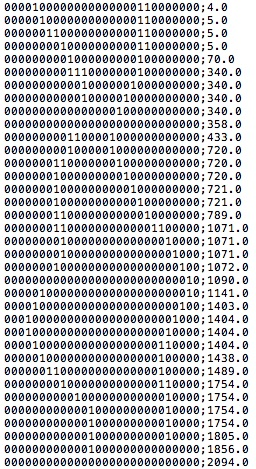
\includegraphics[scale=0.7]{images/rawDataExample.jpg}
\caption{Example of the raw data of one gesture. On the left-hand side the sensor input and on the right the time stamps in milliseconds.}
\label{fig:rawDataExample}
\end{figure}\mnote{Use a filter algorithm to reduce the data}Since more than one vertical and horizontal pinstripe can be connected at the same time we apply a filter algorithm. This filter algorithm takes all x-coordinates and calculates the average and the same for the y-coordinates. The resulting triple composed of the coordinate and the time stamp is added to an \emph{Arraylist} buffer. This is done for all input sets except for all those, who only consists of \emph{0's}. There are two reasons for filtering the input data. The first is the resilience to noise caused by unintended connections or slow separation of the pinstripe layers. The second reason is fact that it is easier for implementing gesture recognition. Apart from this the user intends to press only one point at the sensor.
\\
When a gesture starts we take the coordinates and subtract them from all filtered coordinates of this gesture. Therefore every gesture starts at $(0,0)$ regardless where it is performed on the sensor. This is done for the graphical representation of the strokes and will be useful later on.
\\ \\
\mnote{Implementing mark-based gesture recognition}The next step is to actual recognize easy strokes performed on the prototype.  Since our prototypes have a rather low resolution compared to typical touch input devices we focus on rather simple unistroke gestures. These mark-based gestures are shown in figure \ref{fig:markBasedGestures}. We extend this gestures set by adding 5 gestures. These gestures are a tab and for each swipe gesture we expand it with a swipe in the opposite direction. This leads to a gesture set with 17 simple gestures. \\
\begin{figure}
 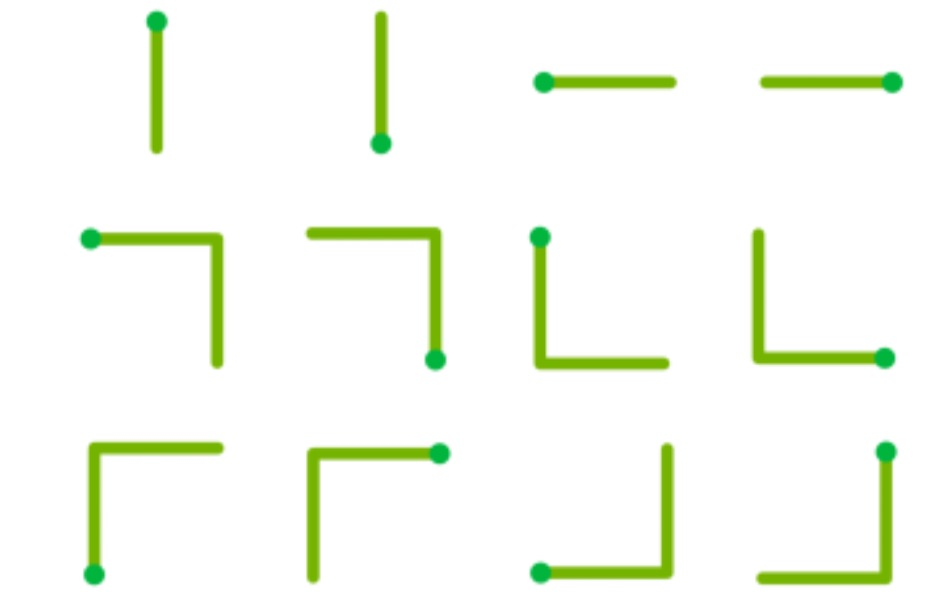
\includegraphics[scale=0.25]{images/markBasedGestures.jpg}
 \caption{Mark-based gestures. Gestures start at the dots. \cite{Bragdon}}
 \label{fig:markBasedGestures}
 \end{figure}Our gesture recognition works as follows. First of all we do not recognize in real-time. We analyze all filtered points, stored in the buffer, after a gesture is considered finished.  Then the algorithm works as follows.
\begin{tt}
\begin{itemize}
\item check for tab
	\begin{itemize}
		\item return $true$ if the size of the buffer is $1$ 
		\item return $true$ if the all coordinates have a $distance$ smaller or equal to $1$ respectively and the time elapsed is smaller than 200 milliseconds
		\item else check for other gestures
	\end{itemize}
\item check for swipe
	\begin{itemize}
	\item assume there is a swipe with the first and the last item of the buffer as terminal points
	\item calculate the $distance$ of the line
	\item return $false$ if the $distance$ is smaller than $3$
	\item for all other points calculate the $distanceToLine$ 
	\item return $false$ if at some index the $distanceToLine$ is greater than $1$
	\item else determine the direction of the swipe and return $true$
	\end{itemize}
\item check for angle
	\begin{itemize}
	\item check if there is a line between the point at $ index - 1$ and last point in the buffer under the exact same conditions applied for swipe
	\item return $false$ if at some index the $distanceToLine$ is greater than $1$
	\item calculate the directions of both lines and return $true$
	\end{itemize}
\item end of checking 
\end{itemize}
\end{tt}
This algorithm classifies each gesture as a tab, swipe, angle, or no gesture. In combination with the directions we calculate for each swipe we can distinguish between all 16 mark-based gestures. The orientation of a line is mapped to one of the four directions up, left, right, or down. Therefore our prototype is resilient to a certain degree of input error. With less effort we can further extend the gesture set by distinguish more directions. 
\\ \\
\mnote{Using 1\$ Unistroke Recognizer for complex gestures}When testing our gesture recognizer with our current prototypes we observe an almost 100\% recognition rate. Based on this finding we decide to go beyond simple mark-based gestures and continue with recognizing  more complex gestures. Therefore we make use of the 1\$ Unistroke Recognizer by \cite{Wobbrock}. This is an easy to implement recognizer which does not require any training data. Providing a template for each gesture is sufficient. A template is an array of consecutive pairs of coordinates. We can pass the coordinates in the filtered buffer straight to the 1\$ recognizer.
\\
This recognizer is orientation independent. Meaning for the marked-based gestures that, without further analysis of orientation, we can only distinguish between a swipe, an angle to the right, and an angle  to the left. However, we can recognize a set of free-form gestures shown in figure \ref{fig:freeFormGestures}.
\begin{figure}
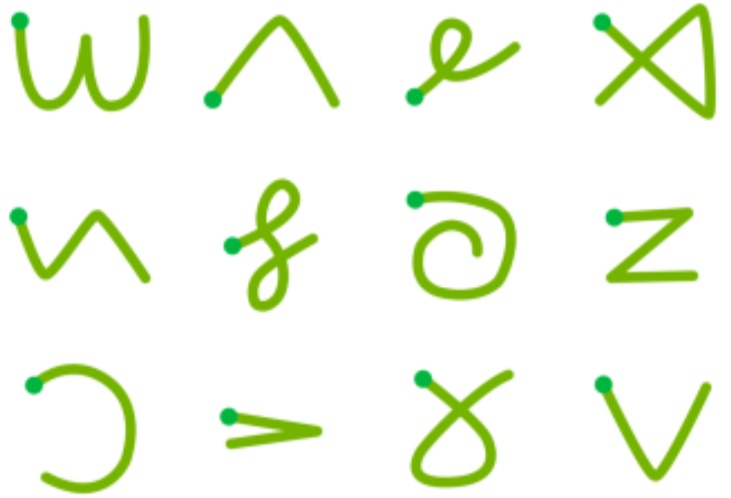
\includegraphics[scale=0.3]{images/freeFormGestures.jpg}
\caption{Free-form gestures \cite{Bragdon}}
\label{fig:freeFormGestures}
\end{figure}


\chapter{System Evaluation}
\label{evaluation}
In this chapter we will evaluate the robustness of our prototype in different extreme conditions.\mnote{Testing the 14 by 14 prototype} We will take a closer look at the performance of the 14 by 14 prototype. Since the prototype is designed as a wearable, we are interested in its behavior under changing conditions. These conditions are composed of softness, curvature, and friction.

\section{Physical Limitation Study}
\mnote{Independent variables: friction, softness, looseness, and curvature}The human body is in motion almost all the time and the clothes we are wearing are not fixed to the skin. This \emph{looseness} and the changing subsurface are variables that may influence the performance of our prototype. Another variable is the \emph{friction} of the overlaying material. Depending on the fabric and method of fashioning, it can, more or less likely, happen that the user slips of the touch-sensing area, or experiences an unpleasant feeling in the operating finger. Furthermore the \emph{softness} of the underlying surface may influence the performance of our prototype. The amount of muscles, adipose tissue, and so forth also differs from human to human. This, in the first place, affects the pressure needed by the user. Then there are the different levels of curvature. Our prototype has flexible spacing-material to separate the pinstripe layer. After a certain amount of bend the material starts creasing, causing some permanent contacts. In this study we will test our prototype in conditions which aim to simulate the in field scenarios. To test to which degree of bend the prototype breaks we used different foams with fixed thickness and different density.

\section{Study Design}
\mnote{conditions}
\mnote{setup}
\mnote{participants}
\mnote{design}The participants had to perform 8 different gestures in different conditions. The set of gestures is shown in figure \ref{fig:gestureTemplate}. To control the curvature, we used aerosol cans with 53mm diameter and 66mm diameter. As a baseline we also used the table with a flat surface. When we tried to perform gestures on a curvature below 53 mm we got permanent contacts immediately. To fixate the aerosol cans we build stands using a laser cutter. The prototype was fixed with duct tape to the surface of the cans. To achieve the curvature with the foam, we used a book and wrapped the foam around the cover and clipped it in a vise. The fabrics (jeans, cotton, rib knit cotton\todo{insert pictures}) were pinned to the prototype with needles. Nevertheless, there is still a certain amount of movement due to the flexibility of the fabrics. The user cannot see the output on the screen. \\
\begin{center}
\begin{figure}
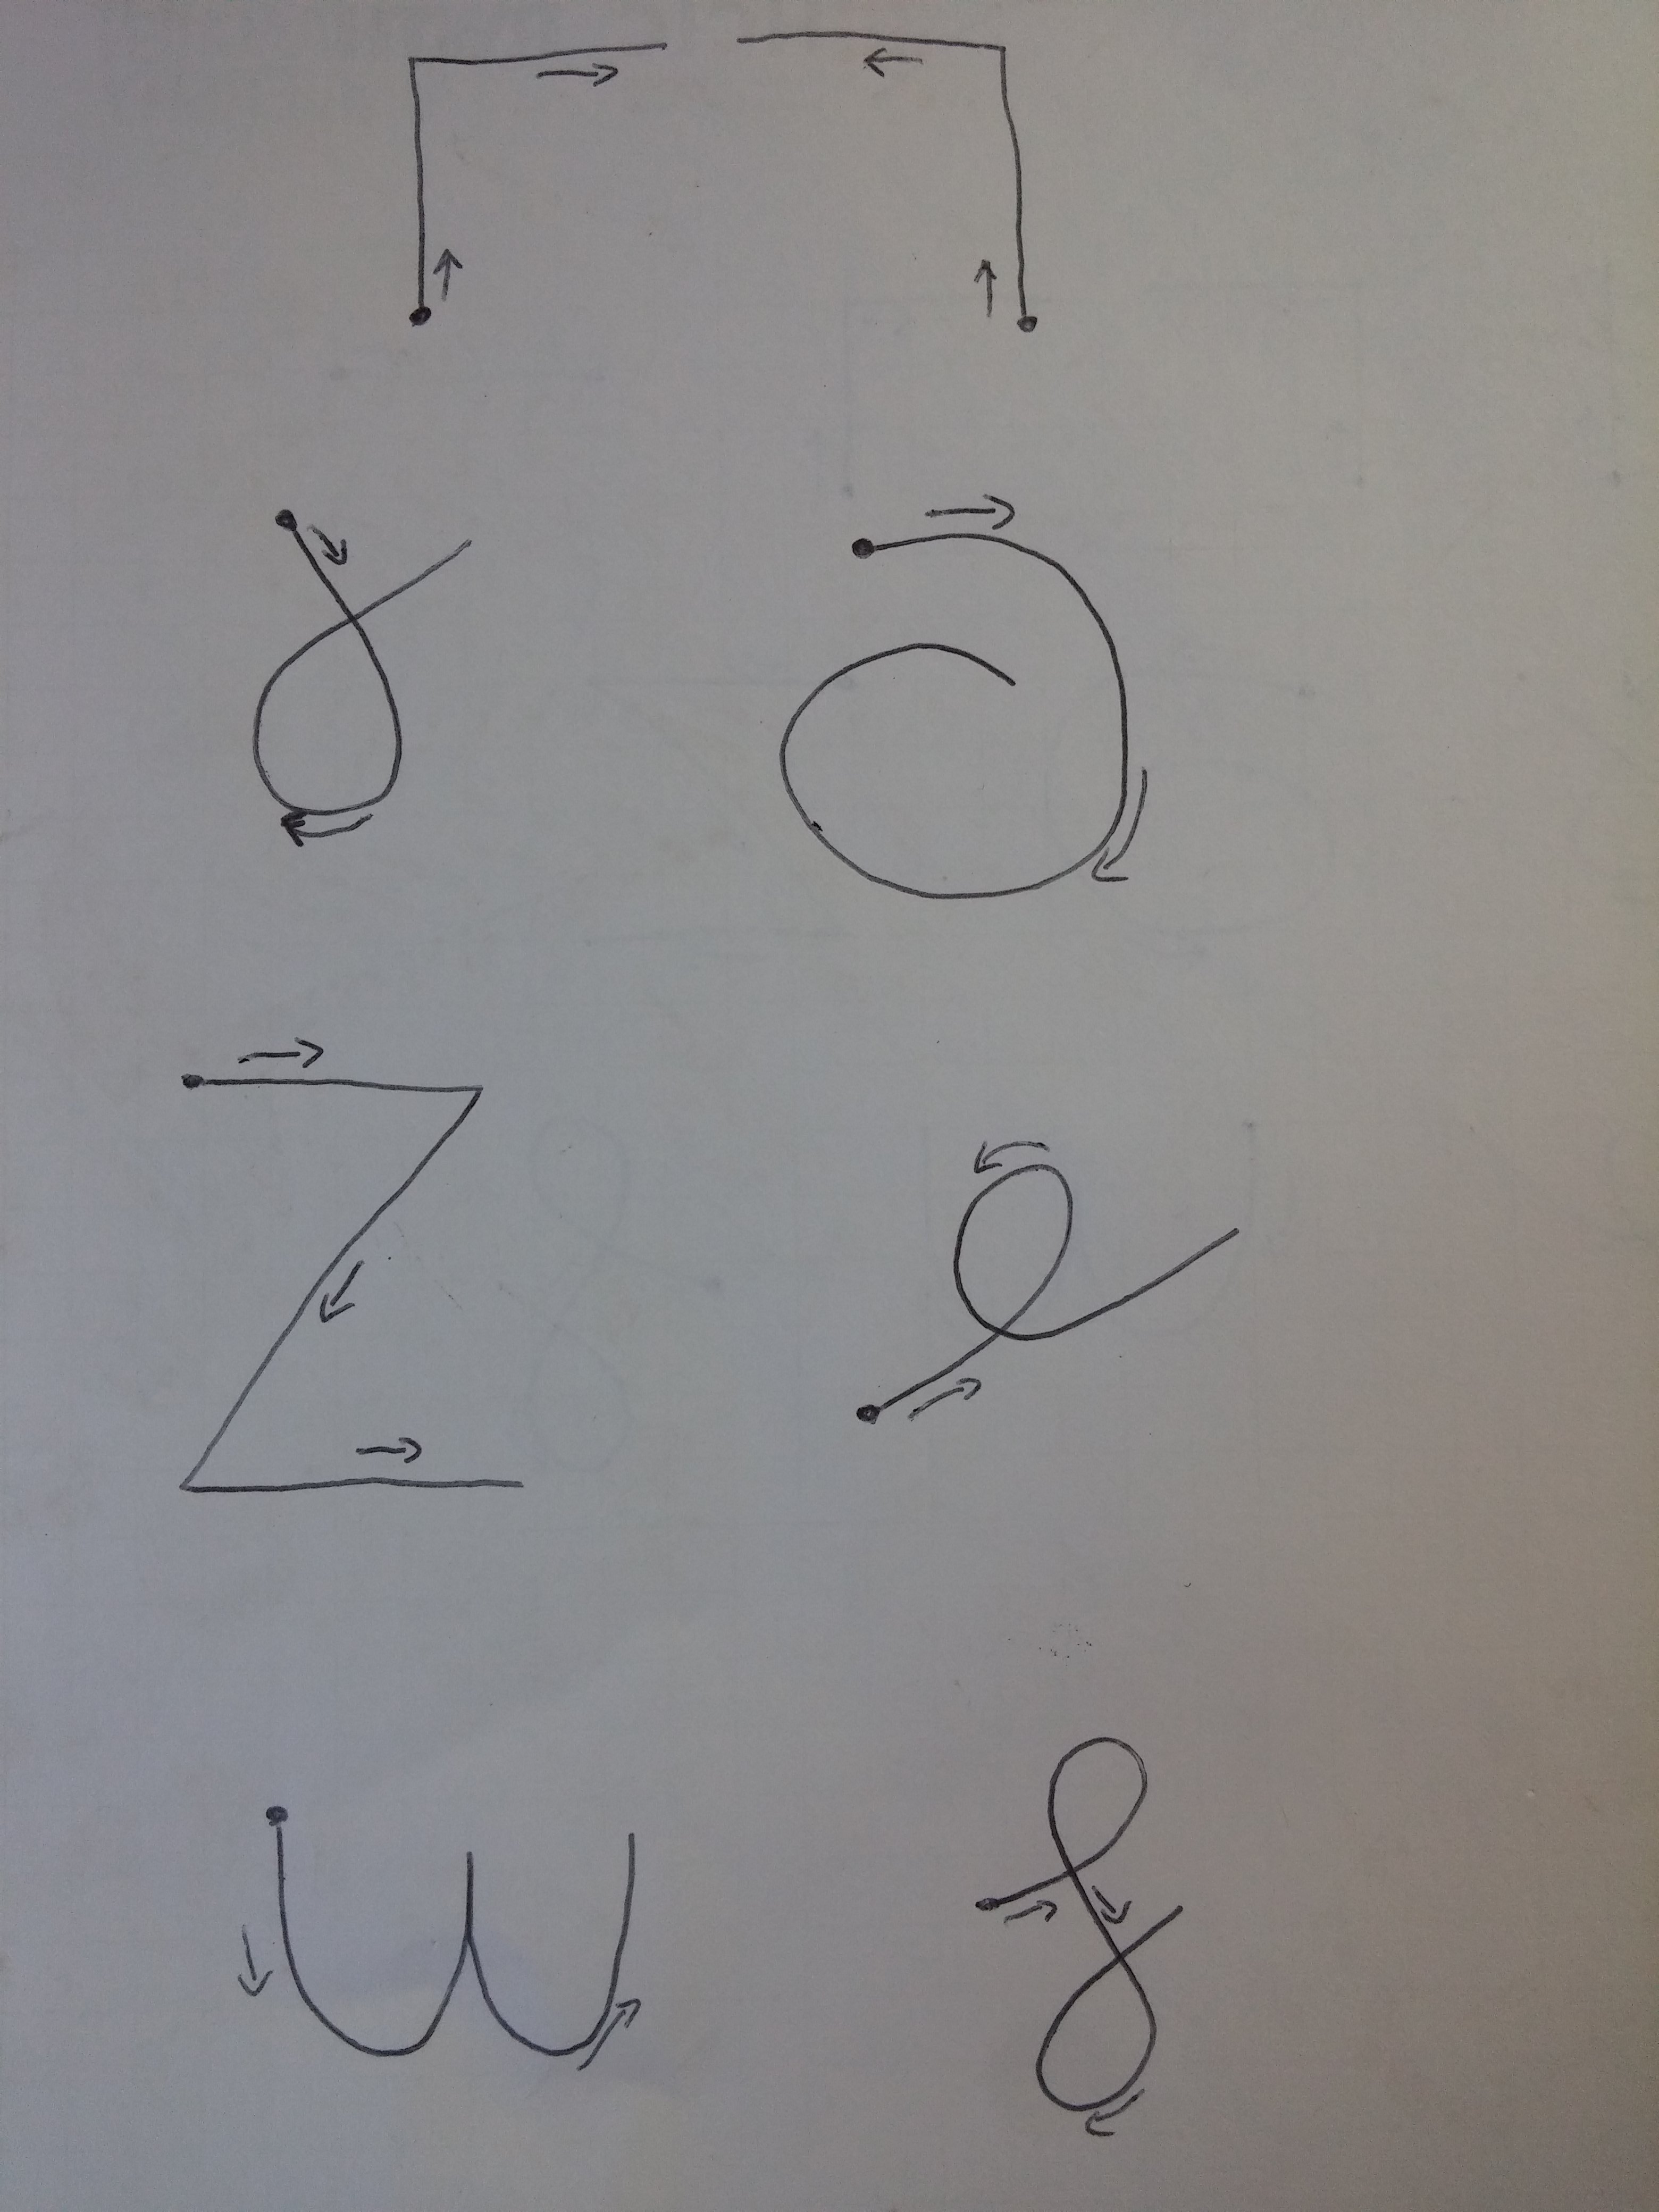
\includegraphics[scale=0.07]{images/gestureTemplate.jpg}
\caption{Gesture set: right angle, left angle, slope, spiral, z, pigtail, w, doubleslope}
\label{fig:gestureTemplate}
\end{figure}
\end{center}
The conditions, at least curvature and softness, were chosen at random. In order to shorten the time of the study, we tested all fabrics consecutively changing the order. Some prior testing has shown that the foam with a density of 1000m$^3$ and 1500m$^3$ perform alike. Thus we dropped the harder foam with 1500$^3$ after the first participant tested both foams in one condition without differences in terms of input error. \\
We asked two right-handed participants, one male (24) and one female (22). One had no experience with wearable where the other was working with wearable computing. The participants were filmed while interacting with the prototype. Furthermore the screen with the application was captured to determine by eye, whether the gesture was recognized correctly or, if not, should have been recognized correctly. Additionally, our program created two log-files for each condition. One logged the filtered data and one the raw sensor data. Both files logged the time stamps of each data point.

\section{Study Procedure}
After the user arrived we introduced her to our prototype. We explained the basic functionality and demonstrated how the output looks like. Then we let the user test the eight gestures and some freestyle strokes. This was done without foam or any additional fabric. We pointed out that a certain amount of pressure is essential for our prototype to recognize the touch. When they felt familiar enough, about 2 minutes of testing, we prepared the first condition. 
\\ \\
For each condition we setup a GoPro Hero 3 to capture the prototype and the acting hand of the user. When we were ready to start recording the screen and setup, we told the user to continue. Since the user cannot see the output during the study, we told the user when insufficient  pressure was applied or when the touch-sensing area was left. In both cases we most likely recognized one or two wrong gestures. We represent the number of wrong gestures with an \emph{x} in the respective chart. 
\\ \\
When one condition is completed we asked the user about their impressions of the fabric, softness, and curvature. 

\section{Observation}
The results proof the general applicability of our prototype. The overall success rate of performed gesture is shown in figure \ref{fig:overallRecognition}. We distinguish between the hardware results by eye, with recognition, and with repetition if the user left the touch sensing area. 84,5\% of all gestures generated recognizable data. Meaning that by eye the output of the data matches the current gesture. However only 75,5\% of these gestures were recognized correctly using the 1\$ recognizer.  One example of a false negative is shown in figure \ref{falsenegative}. Therefore we made this separation, since we are interested in the capabilities of our hardware prototype. Therefore we let the participants repeat those trials, where they  left the touch sensing area. This leads to an average success rate of 87.5\% and the second user even achieved 91\%.
\begin{figure}
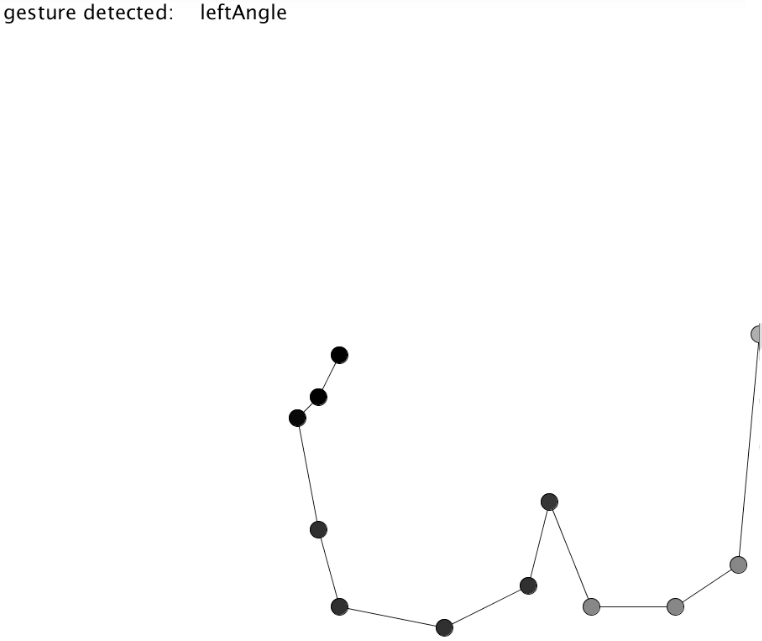
\includegraphics[scale=0.35]{images/falsenegative.jpg}
\caption{The characteristics of \emph{w} are there, but nonetheless \emph{leftAngle} was detected.}
\label{fig:falsenegative}
\end{figure}
\begin{figure}
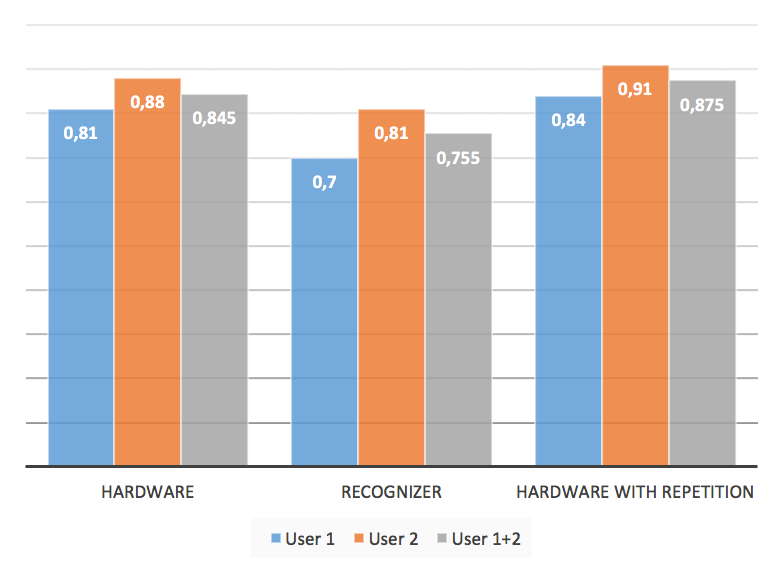
\includegraphics[scale=0.35]{images/overallRecognition.jpg}
\caption{Success rate of all performed gestures with different criteria.}
\label{fig:overallRecognition}
\end{figure}
\\
The difference of hardware success rate and recognizer success rate is almost the same for all conditions. Since we are interested in the performance of the hardware we only consider the success rate of the hardware from now on. 
\\ \\
\mnote{flat surface is best, 53mm worst}
When it comes to surface curvature we got the results we expected shown in figure \ref{fig:surface}. The curvature with a 53mm diameter performs worst but still with a success rate of 75,5\%. The best curvature is no curvature at all. On the table both users achieved a success rate above 90\% with an average of 92\%. It is notable that the user with experience obtained a rate of 95\% with 66mm curvature where the other user got 79\%. Nevertheless, the inexperienced user outperformed the other user on the flat surface. 
\\
When we asked the participants which curvature they prefer they agree that the flat surface it most pleasant for touch input and the more curvature, the more likely it happens that they slip off the surface. This leads to unintentional input and thus to more input error. 
\begin{figure}
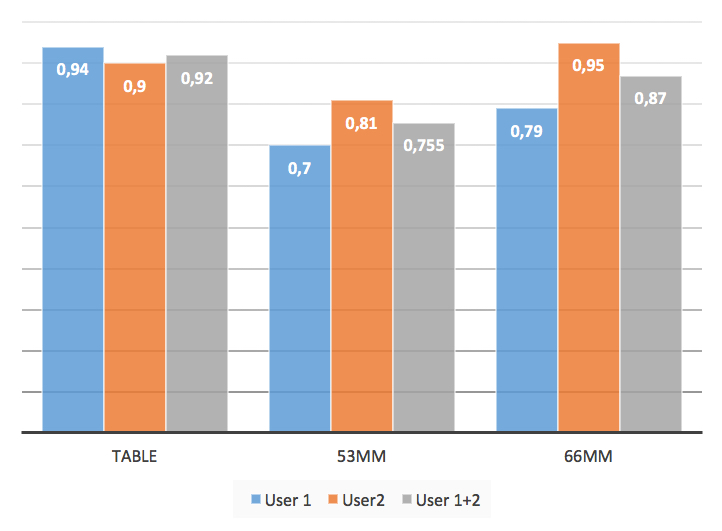
\includegraphics[scale=0.35]{images/surface.jpg}
\caption{Success rates on surface curvatures}
\label{fig:surface}
\end{figure}
\\
The success rates with different softness is shown in figure \ref{fig:foam}. Our hypothesis  that softness has a bad influence on the performance of our prototype was falsified. One user obtained 81\%  in both cases and the more experienced user performed better on the foam (92\%). The participants reported that is was much more pleasant to perform the gestures on the foam due to the distribution of the pressure. 
\\ \\
\begin{center}
\begin{figure}
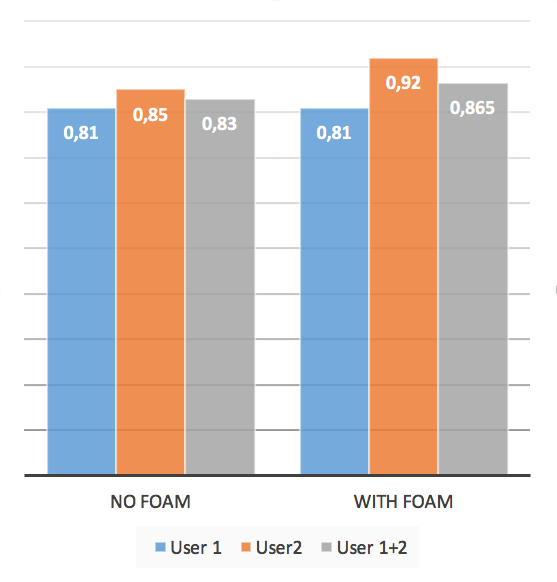
\includegraphics[scale=0.5]{images/foam.jpg}
\caption{Success rates with and without foam}
\label{fig:foam}
\end{figure}
\end{center}
The different materials seem to have no influence on the performance of our prototype as shown in figure \ref{fig:materials}. The average success rate is between 84\% and 86\%. However, the participants reported that the rib knit fabric is extremely annoying due to the immense flexibility. One user said he likes jeans for getting good results but after a while the abrasive surface of the jeans leads to tingle and makes it unpleasant. Both participant prefer cotton and jeans because of their stiffness resulting in less folds. Although the participants reported occasional wrinkles of the rib knit fabric and therefore perceived lose of contact, the sensor still recognized the input as fine as the other fabrics. 
\\ \\
\begin{center}
\begin{figure}
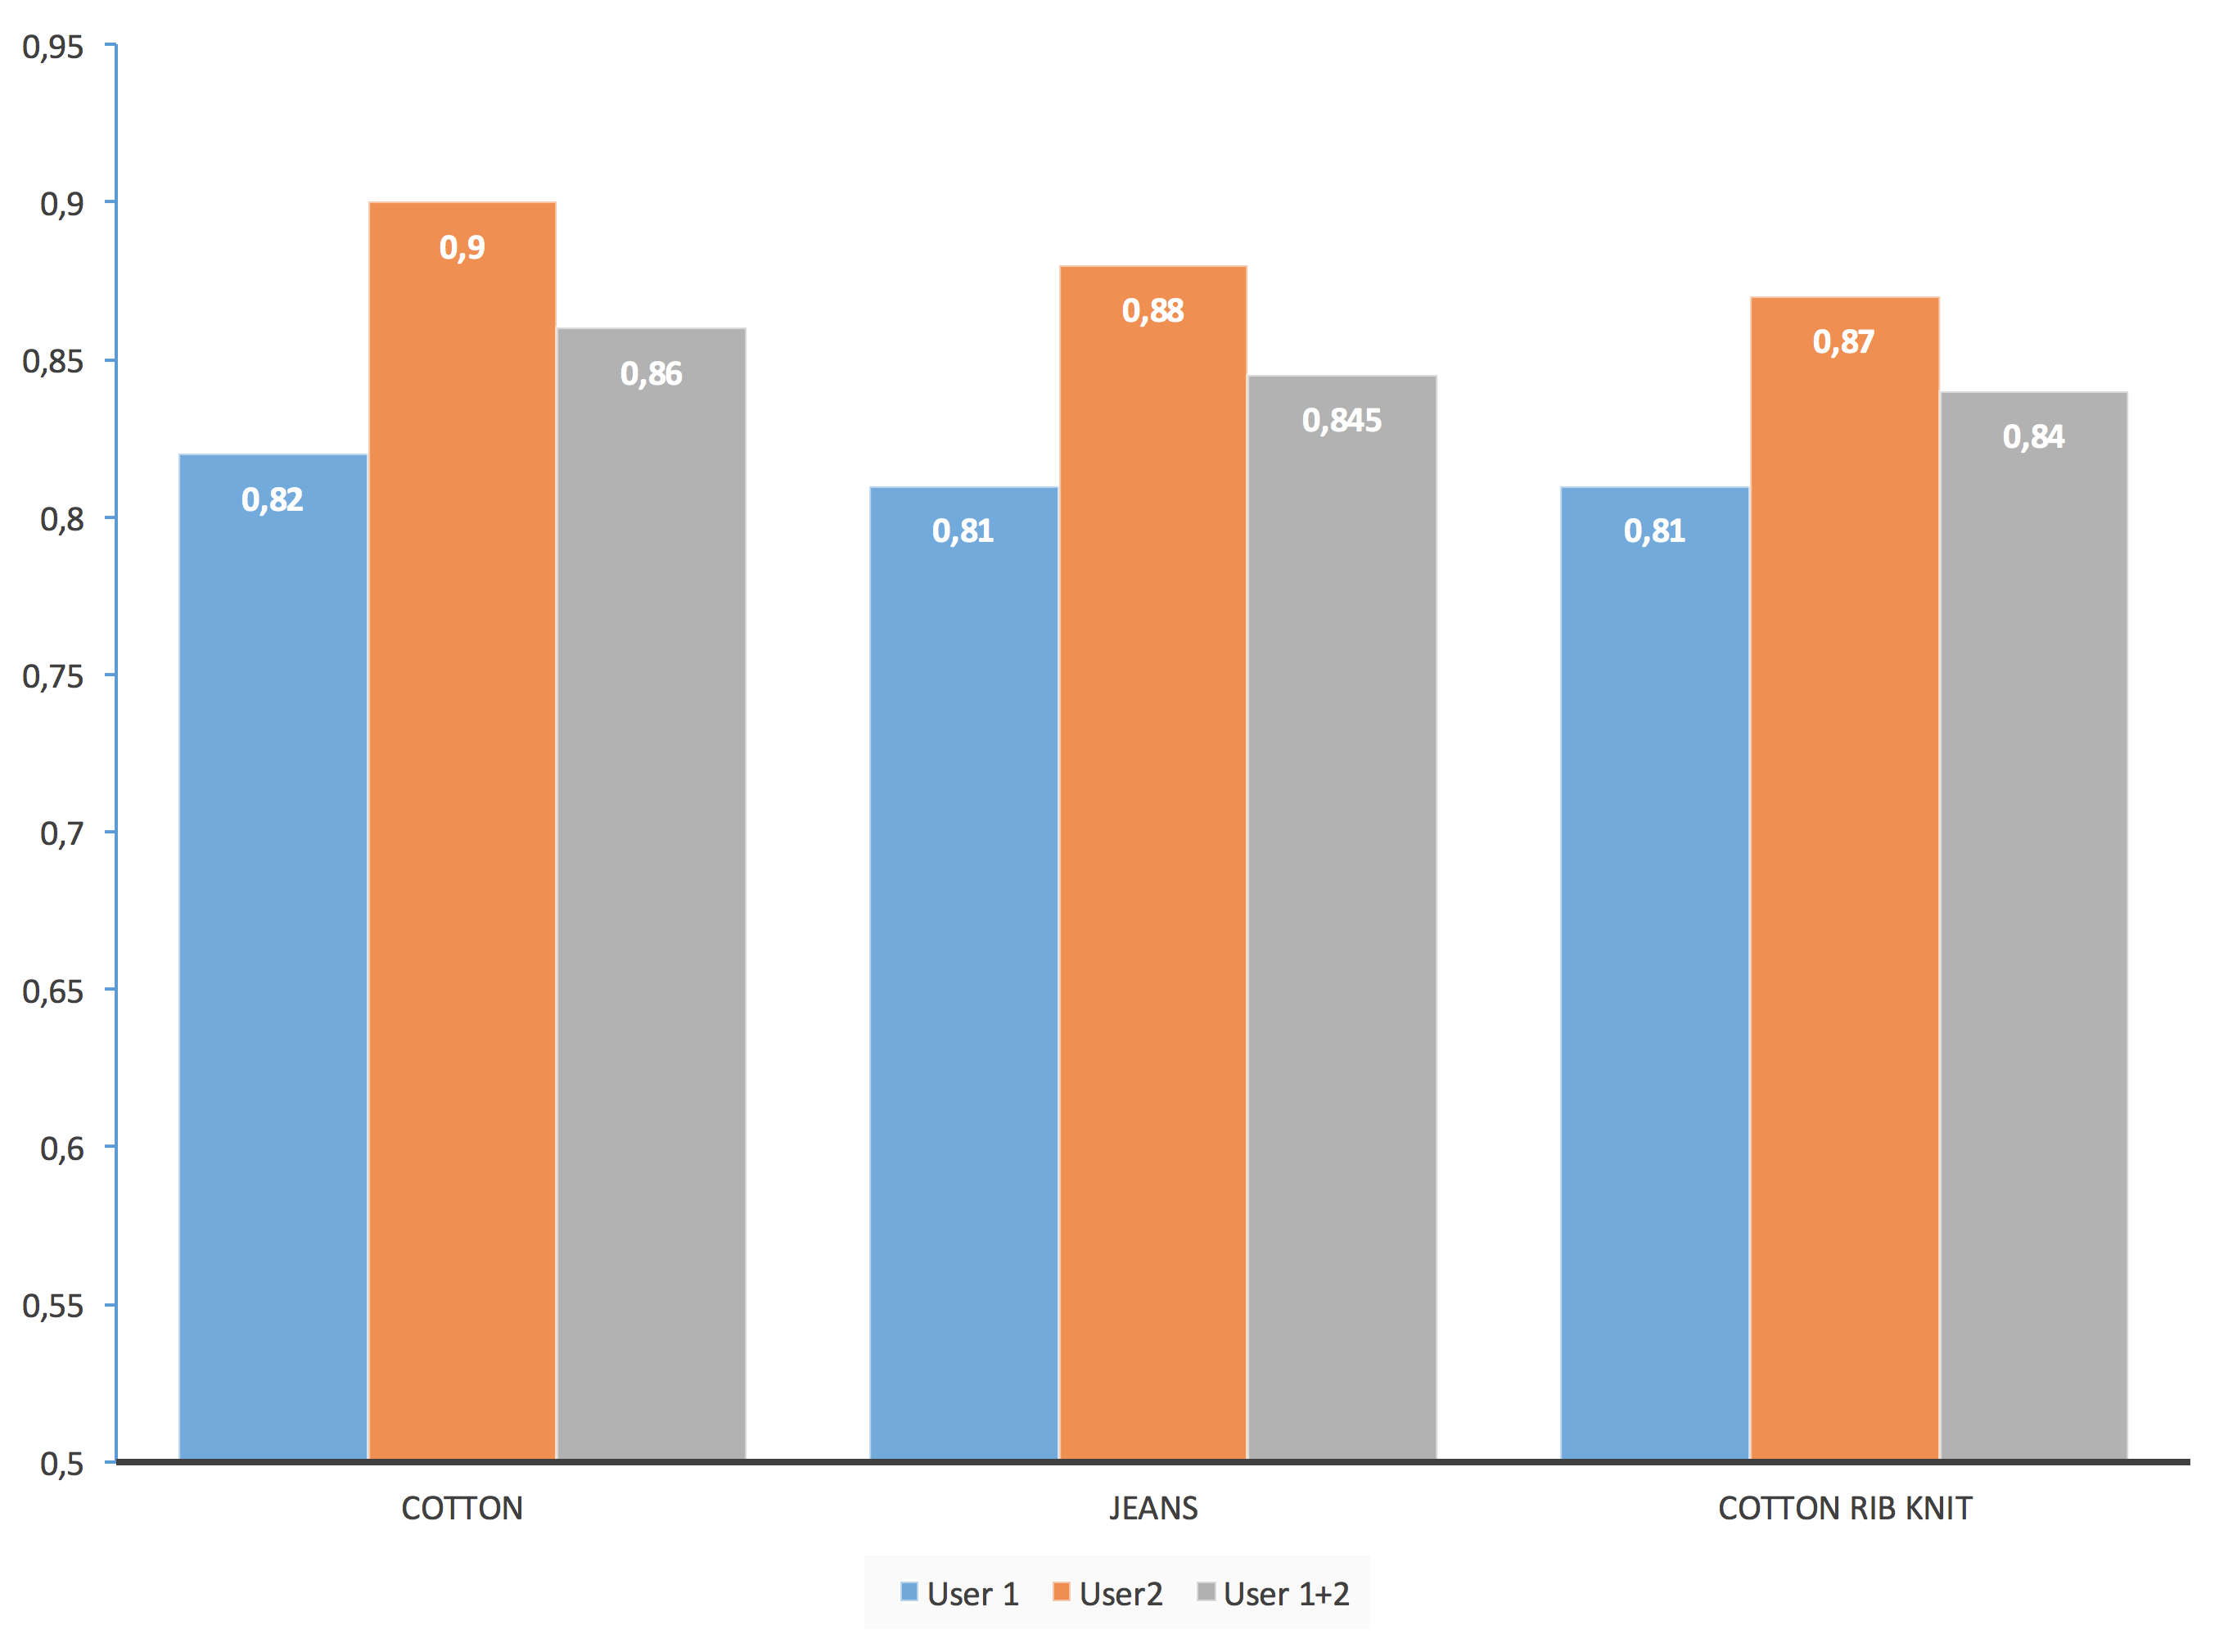
\includegraphics[scale=0.4]{images/materials.jpg}
\caption{Success rates with different materials}
\label{fig:materials}
\end{figure}
\begin{figure}
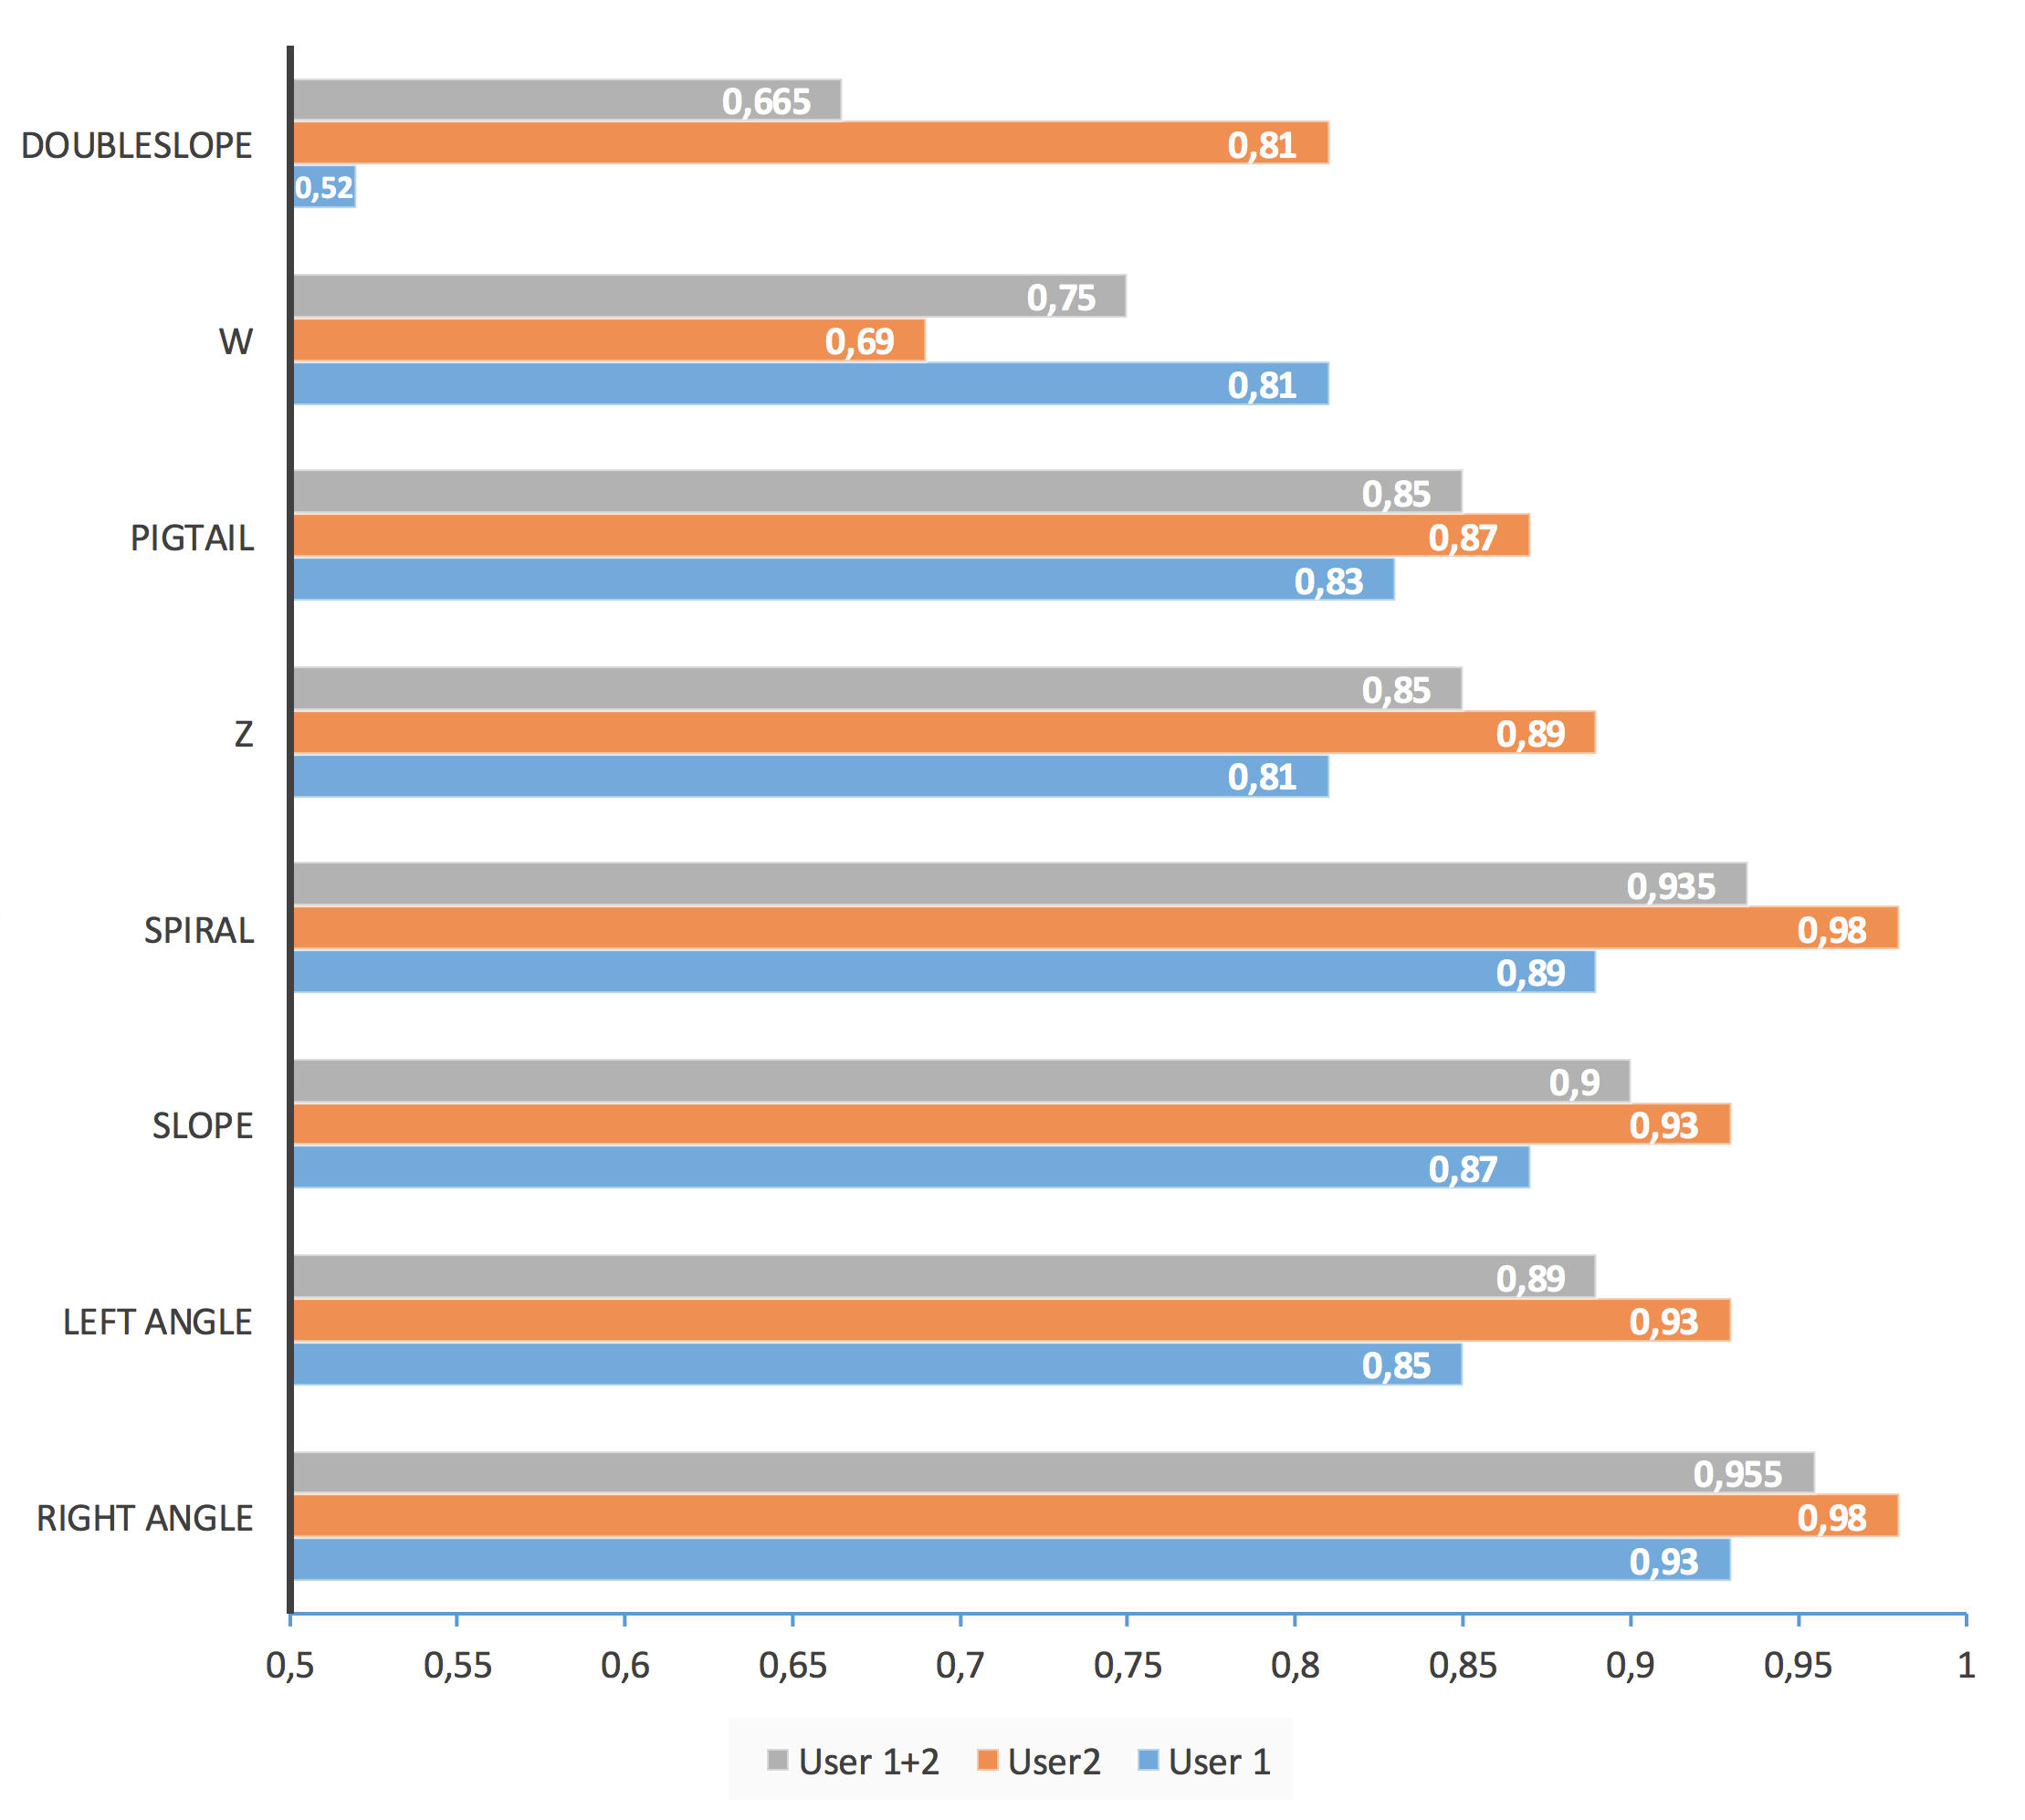
\includegraphics[scale=0.4]{images/gestures.jpg}
\caption{Success rates for each gesture}
\label{fig:gestures}
\end{figure}
\end{center}
The success rates of each gesture is shown in figure \ref{fig:gestures}. The most complex gesture was \emph{doubleslope} and was the hardest gesture to perform with an average success rate of 66,5\%. However the difference between the users is huge (81\% and 52\%). Applying the required amount of pressure steadily is more difficult when the gesture key characteristics are complex. The \emph{doubleslope} gesture requires more changes of direction than \emph{pigtail} (average 85\%).
\\
There is notable difference between \emph{left angle} (89\%) and \emph{right angle}, which has the best  average success rate of 95,5\%. It remains to test if this is ascribed to the dominant hand. Except for the \emph{w} gesture (75\%), the rest of the gesture are within 85\% and 93,5\%. 

\section{Conclusion}
There is a consistent difference between the two participants due to the varying level of experience. This indicates a learning effect which also was the subjective impression of both participants. Primarily the required pressure to generate a contact is remembered over time. 
\emptydoublepage
%!TEX root = ./main.tex
%
% This file is part of the i10 thesis template developed and used by the
% Media Computing Group at RWTH Aachen University.
% The current version of this template can be obtained at
% <http://www.media.informatik.rwth-aachen.de/karrer.html>.

\chapter{Summary and future work}
\label{summaryandfuturework}

In this chapter we will give a summary of our contribution to the field of human computer interaction. Reviewing the hardware and its capabilities will point us to constitutive ideas for future work.

\section{Summary and contributions}
\label{summaryandfuturework.summary}
We presented a 2D textile touchpad for eyes free interaction with novel properties compared to the latest prototypes in this field. It is based on the simple principles of resistive touch technology which has some advantages over capacitive technology when it comes to wearable touch sensing. We presented several related touch pad prototypes in chapter~\ref{relatedwork}. Most of them use capacitive touch and the gestures they are able to detect are rather limited due to the noise generated by the human body. Our prototype only yields a touch if the layers are physically connected. \emph{Grabrics} uses resistive touch as well but the interaction design differs from simple 2D touch. 
\\ \\
In chapter~\ref{Hardware Prototype and Software Development} we described how we built our prototype with low cost materials. The touch pad itself is made out of textiles only making it bendable and breathable, but limit the stretchability of the sensor at the same time. We explained step by step how to attach the pinstripe fabric layers to the spacing material, such that everyone is able to rebuild it in short time. The necessary code is linked in the \ref{appendix}ppendix. Our prototype is easy scalable and is only limited in the number of pins of the used microcontroller. Although we made our prototypes equilateral, it is simply possible to give it any rectangular size. We want to note that a lot of testing of the 14 by 14 was done prior to the user study. 
\\
Furthermore we explained the software for our sensor to detect simple unistroke mark-based gestures using our own recognizer. Then we went one step further and even recognized more complex unistroke free-form gestures. This is the first full textile touch pad being able to do that consistently. An informal user study, presented in chapter~\ref{evaluation}, has shown that. 
We let two participants test the prototype under multiple conditions to evaluate the physical limitations of the sensor. We found that there is a learning effect since we observed better results from the more experienced user. 
\\
Beside that we found that the 1\$ recognizer is not optimal for sensors with a rather low resolution of 14 by 14. Curvature seems to have only significant impact on the overall performance which makes the thigh best suited additional to the fact that both participants prefer jeans fabric for interacting with the sensor. Although both participants liked operating the sensor, both agree that it gets unpleasant over time it it would be best suited for occasional use.

\section{Future work}
\label{summaryandfuturework.futurework}
\index{future work|}
Since the results of the hardware evaluation have shown that our technique of building a 2D textile touchpad is promising, the most immediate step would  be making the sensor actually wearable by integrating it into everyday clothing. This yields new challenges beside recognizing 2D touch. The wiring of sensor and microcontroller and the power supply should be imperceptible. Furthermore the data processing and gesture recognition should be ported to the microcontroller. 
\\ \\
A number of embedded prototypes could be built with a larger range of fabrics used in today's clothing. Then a series of user studies could be conducted to test the performance of the sensor in daily use. There are numerous aspects that impair the performance of the sensor we did not test yet. Applying the required amount of force to your thigh in order to generate a touch might be unpleasant.
\\ \\
For gesture recognition it would be interesting to analyze why the 1\$ recognizer does not work that well with our prototype. Exploring other recognizes or implementing our own advanced recognizer could be an option as well. Also increasing the resolution without making the surface larger could increase the reliability of gesture recognition. The lack of feedback is another issue for wearable devices. \cite{6636291} investigated this problem by providing haptic feedback. Getting feedback when acting close the the edge of the sensor area could greatly improve the performance. 
\index{future work|)}

\emptydoublepage
\begin{appendix}
%!TEX root = ./main.tex
%
% This file is part of the i10 thesis template developed and used by the
% Media Computing Group at RWTH Aachen University.
% The current version of this template can be obtained at
% <http://www.media.informatik.rwth-aachen.de/karrer.html>.

\chapter{APPENDIX}
\label{appendix}

Lorem ipsum dolor sit amet, consectetur adipisicing elit, sed do eiusmod tempor incididunt ut labore et dolore magna aliqua. Ut enim ad minim veniam, quis nostrud exercitation ullamco laboris nisi ut aliquip ex ea commodo consequat. Duis aute irure dolor in reprehenderit in voluptate velit esse cillum dolore eu fugiat nulla pariatur. Excepteur sint occaecat cupidatat non proident, sunt in culpa qui officia deserunt mollit anim id est laborum.Lorem ipsum dolor sit amet, consectetur adipisicing elit, sed do eiusmod tempor incididunt ut labore et dolore magna aliqua. Ut enim ad minim veniam, quis nostrud exercitation ullamco laboris nisi ut aliquip ex ea commodo consequat. Duis aute irure dolor in reprehenderit in voluptate velit esse cillum dolore eu fugiat nulla pariatur. Excepteur sint occaecat cupidatat non proident, sunt in culpa qui officia deserunt mollit anim id est laborum.Lorem ipsum dolor sit amet, consectetur adipisicing elit, sed do eiusmod tempor incididunt ut labore et dolore magna aliqua. Ut enim ad minim veniam, quis nostrud exercitation ullamco laboris nisi ut aliquip ex ea commodo consequat. Duis aute irure dolor in reprehenderit in voluptate velit esse cillum dolore eu fugiat nulla pariatur. Excepteur sint occaecat cupidatat non proident, sunt in culpa qui officia deserunt mollit anim id est laborum.Lorem ipsum dolor sit amet, consectetur adipisicing elit, sed do eiusmod tempor incididunt ut labore et dolore magna aliqua. Ut enim ad minim veniam, quis nostrud exercitation ullamco laboris nisi ut aliquip ex ea commodo consequat. Duis aute irure dolor in reprehenderit in voluptate velit esse cillum dolore eu fugiat nulla pariatur. Excepteur sint occaecat cupidatat non proident, sunt in culpa qui officia deserunt mollit anim id est laborum.

\emptydoublepage
%!TEX root = ./main.tex
%
% This file is part of the i10 thesis template developed and used by the
% Media Computing Group at RWTH Aachen University.
% The current version of this template can be obtained at
% <http://www.media.informatik.rwth-aachen.de/karrer.html>.

\chapter{TITLE OF THE SECOND APPENDIX}
\label{app.02}

Lorem ipsum dolor sit amet, consectetur adipisicing elit, sed do eiusmod tempor incididunt ut labore et dolore magna aliqua. Ut enim ad minim veniam, quis nostrud exercitation ullamco laboris nisi ut aliquip ex ea commodo consequat. Duis aute irure dolor in reprehenderit in voluptate velit esse cillum dolore eu fugiat nulla pariatur. Excepteur sint occaecat cupidatat non proident, sunt in culpa qui officia deserunt mollit anim id est laborum.Lorem ipsum dolor sit amet, consectetur adipisicing elit, sed do eiusmod tempor incididunt ut labore et dolore magna aliqua. Ut enim ad minim veniam, quis nostrud exercitation ullamco laboris nisi ut aliquip ex ea commodo consequat. Duis aute irure dolor in reprehenderit in voluptate velit esse cillum dolore eu fugiat nulla pariatur. Excepteur sint occaecat cupidatat non proident, sunt in culpa qui officia deserunt mollit anim id est laborum.Lorem ipsum dolor sit amet, consectetur adipisicing elit, sed do eiusmod tempor incididunt ut labore et dolore magna aliqua. Ut enim ad minim veniam, quis nostrud exercitation ullamco laboris nisi ut aliquip ex ea commodo consequat. Duis aute irure dolor in reprehenderit in voluptate velit esse cillum dolore eu fugiat nulla pariatur. Excepteur sint occaecat cupidatat non proident, sunt in culpa qui officia deserunt mollit anim id est laborum.Lorem ipsum dolor sit amet, consectetur adipisicing elit, sed do eiusmod tempor incididunt ut labore et dolore magna aliqua. Ut enim ad minim veniam, quis nostrud exercitation ullamco laboris nisi ut aliquip ex ea commodo consequat. Duis aute irure dolor in reprehenderit in voluptate velit esse cillum dolore eu fugiat nulla pariatur. Excepteur sint occaecat cupidatat non proident, sunt in culpa qui officia deserunt mollit anim id est laborum.

\emptydoublepage
\end{appendix}

%--------------------------------------------------------------
\backmatter

%Bibliographie
%bibliography
\clearpage
\phantomsection
\addcontentsline{toc}{chapter}{\protect\numberline{}Bibliography}
\bibliography{thesis}
\emptydoublepage

%Index
%index
\markboth{Index}{Index}
\thispagestyle{plain}
\phantomsection
\addcontentsline{toc}{chapter}{\protect\numberline{}Index}
\printindex

%Satzdatum
%date of typesetting
\newpage
\thispagestyle{empty}
\vspace*{\fill}
\hspace*{\fill}{\tiny Typeset \today}

%--------------------------------------------------------------
\end{document}

